\documentclass[11pt]{article}
\usepackage[T1]{fontenc}
\usepackage[utf8]{inputenc}
\usepackage{lmodern}
\usepackage{amsmath,amssymb,amsthm}
\usepackage[letterpaper,margin=1in]{geometry}
\usepackage{microtype}
\usepackage{array,booktabs,capt-of}
\newcolumntype{L}[1]{>{\raggedright\arraybackslash}p{#1}}
\usepackage{alltt,upquote}
\usepackage{tikz}
\usetikzlibrary{decorations.markings}
\usepackage{url}
\usepackage[colorlinks=true,linkcolor=blue!45!black,citecolor=blue!45!black,urlcolor=blue!45!black]{hyperref}

% Lean identifiers: typewriter, breakable at dots, slashes and underscores.
\DeclareUrlCommand\lean{\urlstyle{tt}}
% Visible placeholder for material that must be filled in before circulation.
\newcommand{\tbd}[1]{\textcolor{red!70!black}{[#1]}}

\newtheorem{theorem}{Theorem}[section]
\newtheorem{lemma}[theorem]{Lemma}
\newtheorem{proposition}[theorem]{Proposition}
\newtheorem{corollary}[theorem]{Corollary}
\theoremstyle{definition}
\newtheorem{example}[theorem]{Example}
\newtheorem{problem}[theorem]{Problem}
\theoremstyle{remark}
\newtheorem{remark}[theorem]{Remark}

\newcommand{\Z}{\mathcal{Z}}
\newcommand{\PP}{\mathbb{P}}
\newcommand{\EE}{\mathbb{E}}
\newcommand{\comp}{\operatorname{comp}}
\newcommand{\tr}{\operatorname{tr}}
\newcommand{\lgs}{\log^{*}}
\newcommand{\lgk}[1]{\log^{(#1)}}
\newcommand{\sm}{\setminus}
\newcommand{\half}{\tfrac12}
\newcommand{\cO}{\mathcal{O}}
\numberwithin{equation}{section}
\setlength{\emergencystretch}{2em}

\hypersetup{pdftitle={The number of cycles in a graph and the minimum number of edges in a pancyclic graph},pdfauthor={KNT, Astra, Fable 5.2}}
\title{The number of cycles in a graph\\ and the minimum number of edges in a pancyclic graph}
\author{KNT \and Astra \and Fable 5.2%
\thanks{Astra and Fable~5.2 are language models: GPT-6 Astra and Claude Fable~5.2.
Section~\ref{sec:status} says who did what, and what a machine has checked.}}
\date{Draft of 10 November 2026}

\begin{document}
\maketitle

\begin{abstract}
Let $\psi(r)$ be the largest number of cycles in a graph of cyclomatic number $r$. We prove that
$\psi(r)\sim2^{r-1}$, as Entringer and Slater conjectured in 1981. More precisely, a graph of large
cyclomatic number $r$ has at most $(\half+21/\log_2\log_2\log_2 r)\,2^{r}$ cycles. The best earlier
bound for cubic graphs was $\frac{15}{16}2^{r}$. The new bound determines the leading coefficient.
It gives no numerical improvement for graphs of any practical size.

The proof has two parts. The first is an estimate from KNT's proof that a pancyclic graph on $n$
vertices needs $n+\log_2n+\lgs n+O(1)$ edges, which settled Erd\H{o}s Problem \#1016. Remove a small
union of cycles from a connected graph of large cyclomatic number. Then a uniformly random even
subgraph, restricted to the remaining edges, is a forest with probability at most $\half+o(1)$. The
second part is new. We add chords to the graph, so that a few triangles carry the count, and we
show that the added chords cost nothing.

We also give a short account of the pancyclic theorem and of the estimate, and we prove two
elementary theorems on paths and cycles in graphs of small cyclomatic number. All four theorems of
the paper are formalised in Lean~4.
\end{abstract}


\section{Introduction}\label{sec:intro}

\subsection{The number of cycles}

Graphs in this paper are finite and simple unless we say otherwise. Throughout, $\log$ is the
binary logarithm, $\lgk{j}$ is its $j$-fold iterate, and $\lgs x$ is the least $j\ge0$ with
$\lgk{j}x\le1$.

For a graph $G$, an \emph{even subgraph} is a set of edges that meets every vertex an even number of
times. With symmetric difference as addition, the even subgraphs form a vector space $\Z(G)$ over
$\mathbb{F}_2$, the \emph{cycle space}. Its dimension is
\[
  \beta(G)=|E(G)|-|V(G)|+\comp(G),
\]
where $\comp(G)$ is the number of components. We call $\beta(G)$ the \emph{rank} of $G$. Other names
are cyclomatic number and cycle rank. A \emph{cycle} is a connected $2$-regular subgraph. We
identify a subgraph that has no isolated vertices with its edge set. Then a cycle is a nonzero
element of $\Z(G)$, so a graph of rank $r$ has at most $2^{r}-1$ cycles.

Let $\psi(r)$ be the largest number of cycles in a graph of rank $r$. Entringer and
Slater~\cite{ES} proved that $2^{r-1}<\psi(r)<2^{r}$, and they conjectured that
$\psi(r)\sim2^{r-1}$. They also proved that the maximum is attained by a cubic graph for every
$r\ge3$. Aldred and Thomassen~\cite{AT} proved that $\psi(r)\le\frac{15}{16}2^{r}$, and that a
planar graph of rank $r$ has at most $2^{r-1}+o(2^{r-1})$ cycles. Alahmadi, Aldred, dela Cruz,
Sol\'e and Thomassen~\cite{AACST} proved that a graph with $p$ vertices and $q>2p+3\log(3p)$ edges
has at most $2^{q-p}$ cycles. For a connected graph, $2^{q-p}=2^{r-1}$.

This left the sparse graphs, and in particular the cubic ones. For those, $\frac{15}{16}2^{r}$ was
the best bound when~\cite{HK} was written, and we have found nothing newer. Our main result proves
the conjecture.

\begin{theorem}\label{thm:cycles}
There is $r_1$ such that every graph of rank $r\ge r_1$ has at most
\[
  \Bigl(\frac12+\frac{21}{\lgk{3}r}\Bigr)2^{r}
\]
cycles. Consequently $\psi(r)\sim2^{r-1}$.
\end{theorem}

The theorem determines the leading coefficient of $\psi(r)$. It is not a useful numerical bound.
The bound is below $2^{r}$ only if $\lgk3r>42$, that is, only if $r$ has more than $2^{2^{42}}$
binary digits. It is below $\frac{15}{16}2^{r}$ only if $\lgk3r>48$, and the threshold $r_1$ is not
explicit. Below these thresholds, $\frac{15}{16}2^{r}$ remains the best bound known. The
second-order term of $\psi(r)$ is open as well. The lower bounds are
$\psi(r)\ge2^{r-1}+r^{2}-3r+3$ from~\cite{ES}, and $\psi(r)\ge2^{r-1}+c\,r\,2^{r/2}$ for some $c>0$
and all large $r$ from~\cite{HK}.

\subsection{The forest estimate and the new step}

The proof of Theorem~\ref{thm:cycles} has two parts. The first part is an estimate of
KNT~\cite{KNT}. Fix a subgraph $W$ of $G$. For an even subgraph $\xi$ of $G$ we call
$\xi\sm E(W)$ its \emph{outside part}. If a cycle uses an edge of $W$, then its outside part is a
proper subset of a cycle, so it is a forest. The estimate says that at most about half of all
outside parts are forests.

\begin{theorem}[Forest estimate, KNT~\cite{KNT}]\label{thm:forest}
There is $r_0$ such that the following holds for all $r\ge r_0$. Let $G$ be a connected simple graph
of rank $r$. Let $W\subseteq G$ be a nonempty union of cycles with at most $\sqrt r$ edges and at
most $(\log r)/100$ components. If $\xi$ is a uniformly random element of $\Z(G)$, then
\begin{equation}\label{eq:forest}
  \PP\bigl(\xi\sm E(W)\text{ is a forest}\bigr)\;\le\;\frac12+\frac{20}{\lgk{3}r}.
\end{equation}
\end{theorem}

The value $\half$ has a simple source. Suppose that $W$ meets the rest of $G$ in two vertices $u$
and $v$ only. Then an outside part has even degree at every vertex, or it has odd degree exactly at
$u$ and $v$. There are equally many outside parts of each kind, and one of the first kind is not a
forest unless it is empty (Example~\ref{rem:twoports}). Theorem~\ref{thm:forest} says that no other
way to attach $W$ leaves a larger proportion of forests, up to the error term.

The second part is new. To count the cycles of $G$, we choose a few edges such that only a small
part of the cycle space avoids them all. Every other cycle uses a chosen edge. We want to apply Theorem~\ref{thm:forest} to a union of cycles $W$ that
contains the chosen edges. But the cycles of $G$ through the chosen edges may all be long, and the
theorem needs $W$ to be small. So we add chords to $G$ until every chosen edge lies on a triangle,
and we let $W$ be the union of these triangles. Each chord raises the rank by one, which could cost
a factor of two in the count. It does not: each chord also doubles the set of even subgraphs that
we count (Lemma~\ref{lem:through}), so the added rank cancels exactly.
Section~\ref{sec:cycles} gives this argument, and Section~\ref{sec:forest} proves
Theorem~\ref{thm:forest}.

\subsection{Pancyclic graphs}

Theorem~\ref{thm:forest} was found for another problem. A graph on $n$ vertices is
\emph{pancyclic} if it contains a cycle of every length $3,4,\dots,n$. Let $n+h(n)$ be the least
number of edges of a pancyclic graph on $n$ vertices.

\begin{theorem}[KNT~\cite{KNT}]\label{thm:main}
There is an absolute constant $A$ such that, for every $n\ge3$,
\[
  \log n+\lgs n-A\;\le\;h(n)\;\le\;\lfloor\log n\rfloor+\lgs n+1 .
\]
\end{theorem}

Bondy~\cite{Bondy} stated without proof that $\log(n-1)-1\le h(n)\le\log n+\lgs n+O(1)$. His lower
bound is a count. A connected graph with $n+h$ edges has at most $2^{h+1}-1$ cycles, and a pancyclic
graph needs $n-2$ of them. Griffin~\cite{Griffin} wrote this count out and determined $h(n)$ for
$n\le37$. Problem~\#1016 in Bloom's collection of Erd\H{o}s problems~\cite{Bloom}
asks whether the upper bound is the truth, and whether even $h(n)-\log n\to\infty$.
Theorem~\ref{thm:main} answers both questions. The paper~\cite{KNT} gives more of the history.

Here is how the estimate enters the proof of Theorem~\ref{thm:main}. Let $W$ have rank $t$ and at
least one edge, and sort the cycles of $G$ by their outside parts. Two cycles with the same outside
part differ only inside $W$, so the cycles with a given outside part have at most $|E(W)|$
different lengths. There are $2^{r-t}$ outside parts. Hence
\begin{equation}\label{eq:trivial}
  \text{the cycles of $G$ have at most }|E(W)|\,2^{r-t}\text{ different lengths.}
\end{equation}
Theorem~\ref{thm:forest} improves this by a factor of almost two when $r$ is large.
Section~\ref{sec:lower} applies the improved bound at ranks that grow like a tower of exponentials.
Each level halves the number of lengths that a given rank can supply, so each level costs one more
edge. This gives the term $\lgs n$. Section~\ref{sec:upper} gives the construction for the upper
bound.

\subsection{Two elementary theorems}

The last two results concern graphs of small rank. Their proofs are elementary and do not use
Theorem~\ref{thm:forest}.

\begin{theorem}\label{thm:exact}
\textup{(a)} Let $N$ be a connected graph and let $u\ne v$ be two of its vertices. Then $N$ has at
most $2^{\beta(N)}$ paths from $u$ to $v$. If it has exactly $2^{\beta(N)}$, then each of these paths
has at least $\beta(N)$ edges, and deleting the edges of any one of them leaves a forest.

\textup{(b)} Let $G$ be a connected graph and let $W\subseteq G$ be a subgraph that contains a cycle.
Suppose that every outside part is the outside part of some cycle of $G$. Then $G-E(W)$ has no two
edge-disjoint cycles, and $\beta(G)\le\beta(W)+|V(W)|+3$.
\end{theorem}

Part~(a) is about graphs that attain the largest possible number of paths between two vertices. It
explains the shape of the construction in Section~\ref{sec:upper}. A gadget that turns $k$ units of
rank into $2^{k}$ path lengths has only long paths, so the short cycles must come from a second,
much smaller gadget, and so on. This is the source of the term $\lgs n$ in the construction.

Part~(b) is about the count of cycles by their outside parts. Call an outside part \emph{wasted} if
no cycle has it as its outside part. Part~(b) says that a graph can avoid all waste only while its
rank exceeds the rank of $W$ by at most $|V(W)|+3$. Section~\ref{sec:exact} proves both parts.

\subsection{Authorship and verification}\label{sec:status}

KNT is a person. Astra and Fable~5.2 are language models. Theorems~\ref{thm:forest}
and~\ref{thm:main}, their proofs, and the Lean formalisation of these proofs come
from~\cite{KNT}. KNT obtained them in September 2026 with Astra, and has described that process in
public~\cite{Claim}. In November 2026 KNT asked Fable~5.2 to look for a simpler proof of
Theorem~\ref{thm:forest}. That search did not find one. It found Theorems~\ref{thm:cycles}
and~\ref{thm:exact}. Fable~5.2 wrote the Lean proofs of these two theorems and drafted this paper.
Astra reviewed a draft. KNT directed the work at each step.

\begin{table}[ht]
\centering\small
\renewcommand{\arraystretch}{1.15}
\begin{tabular}{@{}L{4.3cm}L{1.9cm}L{9.2cm}@{}}
\toprule
Statement & Source & Lean declaration (namespace \lean{Erdos1016}) \\
\midrule
Theorem~\ref{thm:cycles}, upper bound & this paper & \lean{cycleCountTheorem},
  \lean{cycleCountTheorem_general} \\
Theorem~\ref{thm:cycles}, $\psi(r)\sim2^{r-1}$ & this paper & \lean{cycleCountAsymptotic} \\
Theorem~\ref{thm:forest} & \cite{KNT} & \lean{ShortProof.fewComponentForestEstimate} \\
Theorem~\ref{thm:main} & \cite{KNT} & \lean{mainTheorem}; the explicit upper bound is
  \lean{Problem1016.upper_bound_integer} \\
Theorem~\ref{thm:exact}(a) & this paper & \lean{twoTerminalTheorem} \\
Theorem~\ref{thm:exact}(b) & this paper & \lean{noWasteTheorem} \\
\bottomrule
\end{tabular}
\caption{The theorems and their formal counterparts at commit \texttt{9de7271} of the
repository~\cite{Repo}.}\label{tab:status}
\end{table}

All four theorems are formalised in Lean~4~\cite{Lean4} with Mathlib~\cite{Mathlib}.
Table~\ref{tab:status} lists the declarations. The Lean kernel accepts their proofs with the axioms
\lean{propext}, \lean{Classical.choice} and \lean{Quot.sound} only. This certifies the formal
statements. It does not certify the prose of this paper. Appendix~\ref{app:lean} prints the formal
statements of Theorems~\ref{thm:cycles} and~\ref{thm:exact}, so that the reader can compare them
with the text. It also gives the commands that repeat the check, names the Lean declaration for
each step, and says where the formal proofs differ from the text.

The examples and the remarks in this paper are not formalised. Appendix~\ref{app:checks} describes
tests of the examples, and of our wording of the proofs, on small graphs.
Appendix~\ref{app:sources} says which sources we read and how we searched the literature. No
referee has read this draft.

\section{Outside parts}\label{sec:count}

Let $W$ be a subgraph of a graph $G$. Put $r=\beta(G)$, $t=\beta(W)$ and $m=|E(W)|$. The map
$\xi\mapsto\xi\sm E(W)$ is linear on $\Z(G)$, and its kernel is $\Z(W)$. So there are $2^{r-t}$
outside parts, and each of them is the outside part of exactly $2^{t}$ even subgraphs. If $\xi$ is
uniform on $\Z(G)$, then its outside part is uniform on the set of outside parts. Let
\[
  p(G,W)=\PP\bigl(\xi\sm E(W)\text{ is a forest}\bigr).
\]
This is the proportion of outside parts that are forests. It is also the proportion of even
subgraphs whose outside part is a forest:
\begin{equation}\label{eq:count}
  \bigl|\{\xi\in\Z(G):\ \xi\sm E(W)\text{ is a forest}\}\bigr|\;=\;p(G,W)\,2^{r}.
\end{equation}

\begin{lemma}[Counting lemma]\label{lem:count}
Let $p=p(G,W)$.
\begin{enumerate}
\item[\textup{(a)}] If a cycle $C$ of $G$ contains an edge of $W$, then $C\sm E(W)$ is a forest.
Hence at most $p\,2^{r}$ cycles of $G$ contain an edge of $W$.
\item[\textup{(b)}] The cycles of $G$ have at most $2^{r-t}\bigl(pm+1-p\bigr)$ different lengths.
\end{enumerate}
\end{lemma}

\begin{proof}
(a) A proper subset of the edge set of a cycle contains no cycle. The second statement follows
from~\eqref{eq:count}, because distinct cycles are distinct even subgraphs.

(b) Let $x$ be an outside part. Suppose first that $x$ is not a forest, and let $C$ be a cycle with
outside part $x$. Then $x$ contains a cycle and $x\subseteq C$, which forces $C=x$. So $x$ accounts
for at most one cycle, and hence for at most one length. Now suppose that $x$ is a forest, and let
$C$ be a cycle with outside part $x$. Then $C$ contains an edge of $W$, because $C$ is not a
forest. The length of $C$ is $|x|+|C\cap E(W)|$, and $1\le|C\cap E(W)|\le m$. So $x$ accounts for
at most $m$ lengths. There are $p\,2^{r-t}$ outside parts that are forests and $(1-p)\,2^{r-t}$
that are not.
\end{proof}

If $W$ has at least one edge, then part~(b) with $p\le1$ gives the bound~\eqref{eq:trivial} of the
introduction. The lemma improves on it when $p$ is less than one.

\begin{example}[Two points of attachment]\label{rem:twoports}
Suppose that $G=W\cup N$, where $W$ and $N$ are connected, have no common edge, and have exactly two
common vertices $u$ and $v$. A \emph{$\{u,v\}$-join} of $N$ is a set of edges of $N$ in which $u$
and $v$ have odd degree and all other vertices have even degree. The outside parts are the
$2^{\beta(N)}$ even subgraphs of $N$ and the $2^{\beta(N)}$ joins of $N$. A nonempty even subgraph
is not a forest. Hence
\[
  p(G,W)\;\le\;\frac{1+2^{\beta(N)}}{2^{\beta(N)+1}}\;=\;\frac12+2^{-\beta(N)-1},
\]
with equality if and only if every join of $N$ is a forest. So when $W$ is attached at two
vertices, the error term in~\eqref{eq:forest} can be replaced by $2^{-\beta(N)-1}$, which is
exponentially small.

For a concrete case, let $N$ be a chain of $k$ four-cycles, each joined to the next at opposite
vertices, and let $u$ and $v$ be the two ends of the chain. Every join of $N$ is a path from $u$ to
$v$, so equality holds. If $W$ is a triangle and $k$ is large, this graph satisfies the hypotheses
of Theorem~\ref{thm:forest}. So the constant $\half$ in~\eqref{eq:forest} cannot be lowered.

Figure~\ref{fig:twoports} shows the case $k=2$. There $\beta(G)=4$ and $\beta(N)=2$. The eight
outside parts are the four even subgraphs of $N$ and the four paths from $u$ to $v$ in $N$. Five of
them are forests, so $p(G,W)=5/8$. Lemma~\ref{lem:count}(a) allows $\frac58\cdot16=10$ cycles
through $W$, and there are nine.
\end{example}

\begin{figure}[ht]
\centering
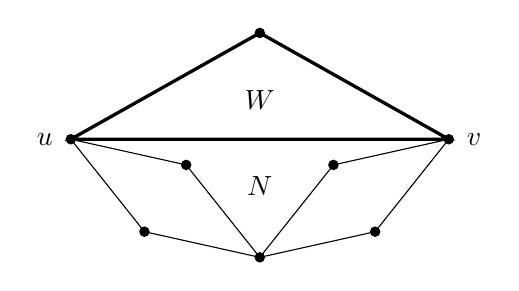
\begin{tikzpicture}
  \coordinate (s) at (0,0);
  \coordinate (t) at (4.8,0);
  \coordinate (m) at (2.4,-1.5);
  \coordinate (w) at (2.4,1.35);
  \coordinate (x1) at (1.465,-0.326);
  \coordinate (y1) at (0.935,-1.174);
  \coordinate (x2) at (3.335,-0.326);
  \coordinate (y2) at (3.865,-1.174);
  \draw (s)--(x1)--(m)--(y1)--cycle;
  \draw (m)--(x2)--(t)--(y2)--cycle;
  \draw[very thick] (s)--(w)--(t)--cycle;
  \foreach \p in {s,t,m,w,x1,y1,x2,y2} \fill (\p) circle (1.9pt);
  \node[left=3pt] at (s) {$u$};
  \node[right=3pt] at (t) {$v$};
  \node at (2.4,0.5) {$W$};
  \node at (2.4,-0.6) {$N$};
\end{tikzpicture}
\caption{The graph of Example~\ref{rem:twoports} for $k=2$: a triangle $W$ (thick) and a chain $N$
of two four-cycles.}
\label{fig:twoports}
\end{figure}

\section{The number of cycles}\label{sec:cycles}

This section proves Theorem~\ref{thm:cycles}. The new step is Lemma~\ref{lem:through}.
Appendix~\ref{app:lean} names the Lean declaration for each step.

\subsection{The lower bound}

Entringer and Slater proved that $\psi(r)>2^{r-1}$ for $r\ge3$. Their examples are cubic: a cycle of
even length with all its long diagonals. These graphs give
$\psi(r)\ge2^{r-1}+r^{2}-3r+3$~\cite[Corollary~4]{ES}.

A simpler example suffices here. Let $j\ge2$. Take vertices $u_1,\dots,u_j$ and, for each $i$, two
further vertices $x_i$ and $y_i$ that are joined to $u_i$ and to $u_{i+1}$, with indices modulo $j$.
This is a ring of $j$ four-cycles: a chain like $N$ in Figure~\ref{fig:twoports}, closed up. It has
$3j$ vertices and $4j$ edges, so its rank is $j+1$. Its cycles are the $j$ four-cycles and the
$2^{j}$ cycles that pass through all the vertices $u_i$. So $\psi(r)\ge2^{r-1}+r-1$ for $r\ge3$.
The formal proof uses a closed chain of shortcuts from the construction of
Section~\ref{sec:upper} instead, which has rank $j+1$ and at least $2^{j}$ cycles.

\subsection{The upper bound}

In this subsection $G$ is a connected simple graph of rank $r$, and $k$ is an integer with
$1\le k\le r$.

\begin{lemma}[Independent edges]\label{lem:indep}
There is a set $D$ of $k$ edges of $G$ such that exactly $2^{r-k}$ even subgraphs of $G$ contain no
edge of $D$. Every edge of $D$ lies on a cycle of $G$.
\end{lemma}

\begin{proof}
Fix a spanning tree of $G$. Exactly $r$ edges of $G$ lie outside the tree. Let $D$ consist of $k$
of them. The graph $G-D$ contains the tree, so it is connected, and its rank is $r-k$. The even
subgraphs of $G$ that contain no edge of $D$ are the even subgraphs of $G-D$. So there are
$2^{r-k}$ of them. An edge of $D$ lies on a cycle, because the tree contains a path between its
ends.
\end{proof}

\paragraph{Chords and triangles.}
Let $e=uv$ be an edge of $D$. It lies on a cycle, so $v$ has a neighbour $w_e\ne u$. Fix such a
neighbour for each edge of $D$. If $u$ and $w_e$ are not adjacent in $G$, add the edge $uw_e$ and
call it a \emph{chord} (Figure~\ref{fig:chord}). Let $G^{+}$ be the graph that we get when we add
all chords, each of them once, and let $a\le k$ be the number of chords. The graph $G^{+}$ is simple
and connected, and it has the same vertices as $G$. So $\beta(G^{+})=r+a$.

For $e\in D$ let $T_e$ be the triangle of $G^{+}$ with the edges $uv$, $vw_e$ and $uw_e$, and let
$W$ be the union of these triangles. Then $W$ is a nonempty union of cycles of $G^{+}$, with at most
$3k$ edges and at most $k$ components. It contains every edge of $D$ and every chord. Every chord
$f$ lies on a triangle $T_f$ of $W$ whose other two edges are edges of $G$. If there are several
such triangles, fix one of them.

\begin{figure}[ht]
\centering
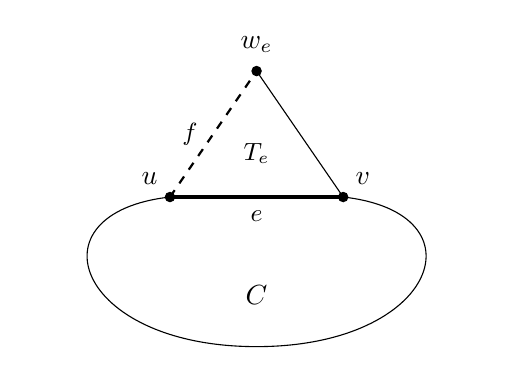
\begin{tikzpicture}
  \coordinate (u) at (0,0);
  \coordinate (v) at (2.2,0);
  \coordinate (w) at (1.1,1.6);
  \draw (v) .. controls (4.0,-0.2) and (3.4,-1.9) .. (1.1,-1.9)
            .. controls (-1.2,-1.9) and (-1.8,-0.2) .. (u);
  \draw[very thick] (u) -- node[below=1pt] {\small$e$} (v);
  \draw (v) -- (w);
  \draw[dashed,thick] (u) -- node[left=2pt] {\small$f$} (w);
  \foreach \p in {u,v,w} \fill (\p) circle (1.9pt);
  \node[above left=1pt] at (u) {$u$};
  \node[above right=1pt] at (v) {$v$};
  \node[above=3pt] at (w) {$w_e$};
  \node at (1.1,-1.25) {$C$};
  \node at (1.1,0.55) {\small$T_e$};
\end{tikzpicture}
\caption{An edge $e=uv$ of $D$, a second neighbour $w_e$ of $v$, and the chord $f=uw_e$ (dashed).
The chord is added if $u$ and $w_e$ are not adjacent in $G$. A cycle $C$ through $e$ and the even
subgraph $C+T_e$ have the same edges outside the triangle $T_e$.}
\label{fig:chord}
\end{figure}

\begin{lemma}[Cycles through $D$]\label{lem:through}
At most $p(G^{+},W)\,2^{r}$ cycles of $G$ contain an edge of $D$.
\end{lemma}

\begin{proof}
Let $F$ be the set of chords, so $|F|=a$. For a cycle $C$ of $G$ that contains an edge of $D$, and
for a set $S\subseteq F$, put
\[
  C_S=C+\sum_{f\in S}T_f .
\]
This is an even subgraph of $G^{+}$. We show two things.

\emph{The outside part of $C_S$ is a forest.} All triangles lie in $W$, so
$C_S\sm E(W)=C\sm E(W)$. The cycle $C$ contains an edge of $D$, and $D\subseteq E(W)$. So
$C\sm E(W)$ is a forest by Lemma~\ref{lem:count}(a).

\emph{The even subgraph $C_S$ determines the pair $(C,S)$.} The cycle $C$ contains no chord. The
triangle $T_f$ contains the chord $f$ and no other chord. So the set of chords in $C_S$ is $S$. Thus
$C_S$ determines $S$, and then it determines $C=C_S+\sum_{f\in S}T_f$.

Let $q$ be the number of cycles of $G$ that contain an edge of $D$. The sets $C_S$ are $q\,2^{a}$
distinct even subgraphs of $G^{+}$ whose outside part is a forest. By~\eqref{eq:count}, applied to
$G^{+}$ and $W$, there are exactly $p(G^{+},W)\,2^{r+a}$ such even subgraphs. Hence
$q\le p(G^{+},W)\,2^{r}$.
\end{proof}

\begin{proof}[Proof of Theorem~\ref{thm:cycles}]
Let $G$ be a graph of rank $r$, where $r$ is large. If $G$ is not connected, add a new vertex and
join it to one vertex of each component. The new edges are bridges, so the rank and the set of
cycles do not change. So we may assume that $G$ is connected.

Let $k$ be the least integer with $2^{k}>\log r$. Then $k\le\log\log r+1$, and $1\le k\le r$. Take
$D$ as in Lemma~\ref{lem:indep}, and take $G^{+}$ and $W$ as above. A cycle of $G$ avoids $D$ or
contains an edge of $D$. At most $2^{r-k}<2^{r}/\log r$ cycles avoid $D$, by
Lemma~\ref{lem:indep}. At most $p(G^{+},W)\,2^{r}$ cycles contain an edge of $D$, by
Lemma~\ref{lem:through}.

It remains to bound $p(G^{+},W)$. The graph $G^{+}$ is connected and simple, and its rank
$r^{+}=r+a$ is at least $r$. The subgraph $W$ is a nonempty union of cycles. It has at most
$3k\le\sqrt{r}\le\sqrt{r^{+}}$ edges and at most $k\le(\log r)/100\le(\log r^{+})/100$ components,
because $r$ is large. So Theorem~\ref{thm:forest} applies to $G^{+}$ and $W$, and
\[
  p(G^{+},W)\;\le\;\frac12+\frac{20}{\lgk3r^{+}}\;\le\;\frac12+\frac{20}{\lgk3r}.
\]
Altogether, the number of cycles of $G$ is at most
\[
  \Bigl(\frac12+\frac{20}{\lgk3r}+\frac1{\log r}\Bigr)2^{r}
  \;\le\;\Bigl(\frac12+\frac{21}{\lgk3r}\Bigr)2^{r},
\]
because $\lgk3r\le\log r$. Together with the lower bound, this gives $\psi(r)\sim2^{r-1}$.
\end{proof}

\begin{remark}\label{rem:chords}
The choice of $k$ is not delicate. The proof needs $2^{-k}\le1/\lgk3r$ for the cycles that avoid
$D$, and $100k\le\log r$ for the components of $W$.

The chords are the point of the proof. Without them one would take for $W$ a union of cycles of $G$
through the edges of $D$. Such cycles can be long, and Theorem~\ref{thm:forest} needs $W$ to be
small. To shorten them one would have to pass to a cubic multigraph and search for short cycles
there. The chords create the short cycles directly, and Lemma~\ref{lem:through} shows that they cost
nothing.
\end{remark}
\section{The lower bound for pancyclic graphs}\label{sec:lower}

This section derives the lower bound of Theorem~\ref{thm:main} from Theorem~\ref{thm:forest}. The
plan is as follows. A number $\Phi(R)\le1$ measures how well a graph of rank at least $R$ can fill
an interval of cycle lengths. In a graph with many cycle lengths we find a small subgraph $W$ that
already contains the short cycles. The forest estimate for $W$ then shows that $\Phi$ drops by a
factor of almost two when the rank grows from $R$ to $2^{256R}$.

For an integer $R\ge1$ let
\[
  \Phi(R)=\sup\,\frac{L-2}{2^{\beta(G)}} ,
\]
where the supremum is over all simple graphs $G$ with $\beta(G)\ge R$ and all integers $L\ge2$ such
that $G$ contains a cycle of each length $3,\dots,L$. A graph of rank $\beta$ has at most
$2^{\beta}-1$ cycles, so $\Phi(R)\le1$. The function $\Phi$ is non-increasing, because a larger $R$
allows fewer graphs.

\begin{lemma}[Witness]\label{lem:witness}
Let $R\ge1$ and $\varphi=\Phi(R)$, and let $G$ contain a cycle of each length $3,\dots,L$, where
$L\ge2^{2R}$. Then $G$ has a subgraph $W$ that is a union of at most $2R$ cycles, with
$\beta(W)\ge2R$ and $|E(W)|\le\varphi\,2^{2R}+2^{R}+5R$.
\end{lemma}

\begin{proof}
Put $W_0=\emptyset$ and $W_{i+1}=W_i\cup C_i$, where $C_i$ is a cycle of $G$ whose length $\ell_i$ is
the least integer $\ge3$ that is not the length of a cycle of $W_i$. Stop as soon as the rank is at
least $2R$. Consider a step, and let $s=\beta(W_i)<2R$. The graph $W_i$ contains cycles of the
$\ell_i-3$ lengths $3,\dots,\ell_i-1$. Therefore $\ell_i-3\le2^{s}-1$. This gives
$\ell_i\le2^{2R-1}+2\le L$, so $C_i$ exists. If $s\ge R$, then also $\ell_i-3\le\varphi\,2^{s}$, by
the definition of $\Phi$. The cycle $C_i$ is not a subgraph of $W_i$, so the rank increases at every
step. So there are at most $2R$ steps, their ranks $s$ are distinct, and
\[
  |E(W)|\;\le\;\sum_i\ell_i\;\le\;\sum_{s=0}^{R-1}\bigl(2^{s}+2\bigr)+\sum_{s=R}^{2R-1}\bigl(\varphi\,2^{s}+3\bigr)
  \;\le\;\varphi\,2^{2R}+2^{R}+5R .\qedhere
\]
\end{proof}

\begin{proposition}[Near-halving]\label{prop:halving}
For every sufficiently large integer $R$,
\[
  \Phi\bigl(2^{256R}\bigr)\;\le\;\Bigl(\frac12+\frac{20}{\lgk{2}R}\Bigr)\Phi(R)+2^{2-R}.
\]
\end{proposition}

\begin{proof}
Let $G$ be a simple graph of rank $r\ge2^{256R}$ with a cycle of each length $3,\dots,L$. We bound
$(L-2)\,2^{-r}$. Identifying a vertex of one component with a vertex of another changes neither the
rank nor the set of cycles, so we may assume that $G$ is connected. If $L<2^{2R}$, then
$(L-2)\,2^{-r}<2^{2-R}$, and we are done.

Otherwise let $W$ be as in Lemma~\ref{lem:witness}, with $m$ edges and rank $t\ge2R$, and let
$\varphi=\Phi(R)$. Then $m\le2^{2R+1}\le\sqrt r$ and $\comp(W)\le2R\le(\log r)/100$. This is
the only place in this proof where the size of the exponent $256$ matters, and any exponent of at
least $200$ would do.
So Theorem~\ref{thm:forest} gives
\[
  p(G,W)\;\le\;\frac12+\frac{20}{\lgk3r}\;\le\;\frac12+\delta,
  \qquad\text{where }\delta=\frac{20}{\lgk2R}.
\]
The second inequality holds because $\lgk3r\ge\log(8+\log R)\ge\lgk2R$. The graph $G$ has cycles of
at least $L-2$ lengths. So Lemma~\ref{lem:count}(b), with $p=p(G,W)$, and the bounds on $t$ and $m$
give
\[
  \frac{L-2}{2^{r}}\;\le\;\frac{pm+1}{2^{t}}
  \;\le\;\Bigl(\frac12+\delta\Bigr)\bigl(\varphi+2^{-R}+5R\,2^{-2R}\bigr)+2^{-2R}
  \;\le\;\Bigl(\frac12+\delta\Bigr)\varphi+2^{2-R}.\qedhere
\]
\end{proof}

\begin{corollary}\label{cor:phi}
There is a constant $c$ such that $\Phi(r)\le c\,2^{-\lgs r}$ for all $r\ge1$.
\end{corollary}

\begin{proof}
Fix $R_0\ge512$ so large that Proposition~\ref{prop:halving} holds for all $R\ge R_0$. Let
$R_{j+1}=2^{256R_j}$ and $\delta_j=20/\lgk2R_j$. By Proposition~\ref{prop:halving}, the numbers
$a_j=2^{j}\Phi(R_j)$ satisfy
\[
  a_{j+1}\;\le\;(1+2\delta_j)\,a_j+2^{\,j+3-R_j}.
\]
For $j\ge2$ we have $\lgk2R_j=8+256R_{j-2}$, so $\sum_j\delta_j<\infty$. Also
$\sum_j2^{\,j-R_j}<\infty$. Hence the numbers $a_j$ are bounded, say $\Phi(R_j)\le c_1 2^{-j}$.

The numbers $R_j$ grow like a tower of exponentials. To bound $\lgs R_j$, we compare them with an
exact tower. Let $U_0=R_0^2$ and $U_{j+1}=2^{U_j}$, so that $\lgs U_j=j+\lgs U_0$. Then
$R_j\le\sqrt{U_j}$ for all $j$. Indeed, if this holds for $j$, then
\[
  R_{j+1}=2^{256R_j}\;\le\;2^{256\sqrt{U_j}}\;\le\;2^{U_j/2}=\sqrt{U_{j+1}},
\]
because $\sqrt{U_j}\ge R_0\ge512$. Hence $\lgs R_j\le j+\lgs U_0$.

Finally let $r\ge R_0$, and let $j$ be largest with $R_j\le r$. Then
$\Phi(r)\le\Phi(R_j)\le c_12^{-j}$ and $\lgs r\le\lgs R_{j+1}\le j+1+\lgs U_0$. Together these give
$\Phi(r)\le c\,2^{-\lgs r}$ with $c=c_1\,2^{1+\lgs U_0}$. For $r<R_0$ use $\Phi(r)\le1$, and enlarge
$c$ if necessary.
\end{proof}

\begin{proof}[Proof of the lower bound in Theorem~\ref{thm:main}]
Let $G$ be a pancyclic graph with $n$ vertices and $n+h$ edges. It is connected, so its rank is
$r=h+1$. By the definition of $\Phi$ and by Corollary~\ref{cor:phi},
\[
  n-2\;\le\;\Phi(r)\,2^{r}\;\le\;c\,2^{\,r-\lgs r}.
\]
We compare $\lgs r$ with $\lgs n$. The trivial bound $n-2\le2^{r}-1$ gives
$n\le2^{r+1}\le2^{2^{r}}$, hence $\lgs n\le\lgs r+2$. Now take logarithms in the display:
\[
  h=r-1\;\ge\;\log(n-2)+\lgs r-\log c-1\;\ge\;\log n+\lgs n-\log c-5.\qedhere
\]
\end{proof}

\paragraph{Formal counterpart.}
In the Lean code $\Phi$ is \lean{actualRankTail}. Proposition~\ref{prop:halving} is
\lean{ShortProof.recurrence_of_few_component_forest_estimate}, with the same constants.
Corollary~\ref{cor:phi} is an instance of \lean{recurrence_logStar_bound}. Lemma~\ref{lem:witness}
corresponds to \lean{ShortProof.exists_budgeted_witness}, where the bookkeeping differs in detail.
\section{The construction}\label{sec:upper}

This section proves the upper bound of Theorem~\ref{thm:main}. The construction follows~\cite{KNT}.
It is a chain of beads. Bead $i$ can be passed in two ways, and the two ways differ in length by
$2^{i}$. So $k$ beads give $2^{k}$ consecutive path lengths for the price of $k$ chords. A few more
chords close shorter and shorter parts of the chain, and these supply the short cycles.

\begin{proposition}\label{prop:upper}
For every $n\ge3$ there is a pancyclic graph with $n$ vertices and at most
$n+\lfloor\log n\rfloor+\lgs n+1$ edges.
\end{proposition}

\begin{proof}
For $3\le n\le6$ take a cycle $u_0u_1\cdots u_{n-1}$, with the chord $u_0u_2$ if $n\ge4$ and also
the chord $u_0u_3$ if $n=6$. Now let $n\ge7$.

\emph{The necklace.} Let $k\ge2$ be the largest integer with $2^{k}+k+1\le n$, so that
$n\le2^{k+1}+k+1$. Let $H$ be a cycle of length $n$, and let $Q\subseteq H$ be a path that is
composed of consecutive segments $Q_0,\dots,Q_{k-1}$, where $Q_i$ has $2^{i}+1$ edges and joins
$v_i$ to $v_{i+1}$. Thus $Q$ has $2^{k}+k-1\le n-2$ edges. Add the chords $e_i=v_iv_{i+1}$ for
$0\le i<k$. For $1\le j\le k$ let $N_j$, the \emph{necklace with $j$ beads}, be the union of
$Q_0,\dots,Q_{j-1}$ and $e_0,\dots,e_{j-1}$ (Figure~\ref{fig:necklace}).

A path from $v_0$ to $v_j$ in $N_j$ uses either $Q_i$ or $e_i$ for each $i<j$, and it is shorter by
$2^{i}$ if it uses $e_i$. So $N_j$ has $2^{j}$ such paths, exactly one of each length from $j$ to
$2^{j}+j-1$. The rest $H-Q$ of the outer cycle is a path from $v_k$ to $v_0$ with $n-2^{k}-k+1$
edges. Together with $N_k$ it contains a cycle of each length in the interval
\[
  [\,n-2^{k}+1,\ n\,].
\]

\emph{Closing chords.} For $2\le j\le k$ the chord $f_j=v_0v_j$ closes the paths of $N_j$ to cycles
of all lengths in the interval
\[
  I_j=[\,j+1,\ 2^{j}+j\,].
\]
Add the chord $f_j$ for $j=k$, then for $j=\lceil\log k\rceil$, and so on: as long as the last
value of $j$ is larger than $2$, the next value is $\lceil\log j\rceil$. The last value is $2$. If
$j'=\lceil\log j\rceil$, then $2^{j'}\ge j$, so the intervals $I_{j'}$ and $I_j$ overlap or are
adjacent. Since $I_2=[3,6]$, these chords give a cycle of each length in $[\,3,\ 2^{k}+k\,]$.

\emph{All lengths.} The intervals $[\,3,\ 2^{k}+k\,]$ and $[\,n-2^{k}+1,\ n\,]$ cover all lengths
from $3$ to $n$, except for the length $2^{k}+k+1$ in the case $n=2^{k+1}+k+1$. In that case add
one more chord, which joins $v_k$ to the neighbour of $v_0$ on $H-Q$. This chord, the edge from that
neighbour to $v_0$, and the path $Q$ form a cycle of length $2^{k}+k+1$.

\emph{The number of chords.} For an integer $j\ge3$ we have $\lgs\lceil\log j\rceil=\lgs j-1$, and
$\lgs2=1$. So exactly $\lgs k$ chords $f_j$ were added. The number of all chords is therefore at
most $k+\lgs k+1\le\lfloor\log n\rfloor+\lgs n+1$.
\end{proof}

\begin{figure}[ht]
\centering
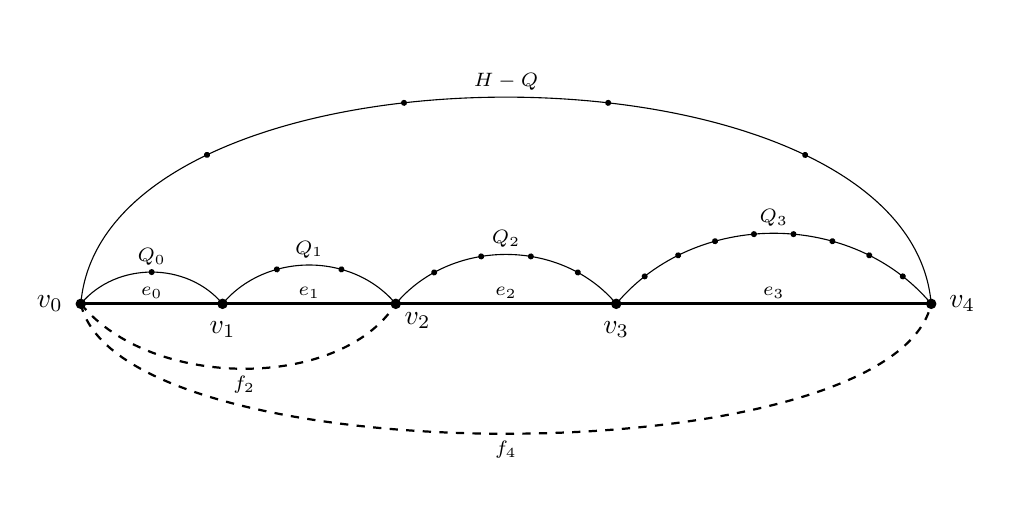
\begin{tikzpicture}[
  iv/.style 2 args={postaction={decorate,decoration={markings,
      mark=between positions #1 and #2 step #1 with {\fill (0,0) circle (1.1pt);}}}}]
  \coordinate (v0) at (0,0);
  \coordinate (v1) at (1.8,0);
  \coordinate (v2) at (4.0,0);
  \coordinate (v3) at (6.8,0);
  \coordinate (v4) at (10.8,0);
  \draw[iv={0.5}{0.51}]    (v0) to[bend left=50] node[pos=0.5,above=-1pt] {\scriptsize$Q_0$} (v1);
  \draw[iv={0.3333}{0.67}] (v1) to[bend left=50] node[pos=0.5,above=-1pt] {\scriptsize$Q_1$} (v2);
  \draw[iv={0.2}{0.81}]    (v2) to[bend left=50] node[pos=0.5,above=-1pt] {\scriptsize$Q_2$} (v3);
  \draw[iv={0.1111}{0.89}] (v3) to[bend left=50] node[pos=0.5,above=-1pt] {\scriptsize$Q_3$} (v4);
  \draw[iv={0.2}{0.81}]    (v0) .. controls (0.3,3.5) and (10.5,3.5) .. node[pos=0.5,above=-1pt] {\scriptsize$H-Q$} (v4);
  \foreach \a/\b/\i in {v0/v1/0,v1/v2/1,v2/v3/2,v3/v4/3}
    \draw[very thick] (\a) -- node[pos=0.5,above=-2pt] {\scriptsize$e_{\i}$} (\b);
  \draw[thick,dashed] (v0) .. controls (0.9,-1.1) and (3.3,-1.1) .. node[pos=0.5,below=-1pt] {\scriptsize$f_2$} (v2);
  \draw[thick,dashed] (v0) .. controls (0.5,-2.2) and (10.3,-2.2) .. node[pos=0.5,below=-1pt] {\scriptsize$f_4$} (v4);
  \foreach \p in {v0,v1,v2,v3,v4} \fill (\p) circle (1.9pt);
  \node[left=3pt] at (v0) {$v_0$};
  \node[below=3pt] at (v1) {$v_1$};
  \node[anchor=north west,inner sep=3pt] at (v2) {$v_2$};
  \node[below=3pt] at (v3) {$v_3$};
  \node[right=3pt] at (v4) {$v_4$};
\end{tikzpicture}
\caption{The construction for $n=24$, where $k=4$. The segments $Q_0,\dots,Q_3$ of the outer cycle
$H$ have $2,3,5,9$ edges and are doubled by the chords $e_0,\dots,e_3$. The chord $f_4$ gives the
cycle lengths $5,\dots,20$, the rest $H-Q$ of the outer cycle gives $9,\dots,24$, and $f_2$ gives
$3,\dots,6$.}
\label{fig:necklace}
\end{figure}

\paragraph{Formal counterpart.}
The Lean theorem \lean{Problem1016.upper_bound_integer} states that
$h(n)\le\lfloor\log n\rfloor+\lgs n+1$ for every $n\ge3$. Its proof formalises the construction
of~\cite{KNT}. The proof above describes that construction in our own words. As a check on the
wording, we built the graph of this section by computer for all $n\le139$ and for eight larger
values up to $522$. Each of these graphs is pancyclic and has at most the stated number of edges
(Appendix~\ref{app:checks}).
\section{Proof of the forest estimate}\label{sec:forest}

This section proves Theorem~\ref{thm:forest}. The argument is that of~\cite{KNT}. It has five steps.
\begin{enumerate}
\item \emph{Cuts.} For a set $A$ of vertices, consider the event that $\xi$ avoids every edge that
leaves $A$. Its probability is explicit. For two disjoint sets the two events are correlated by the
factor $2^{\ell-1}$, where $\ell$ counts the links between the sets (Lemma~\ref{lem:link}). One link
means independence, and two links mean a factor of two.
\item \emph{Reduction.} We pass to a graph $\Gamma$ with all degrees at most $3$, in which $W$ has
become a small set $P$ of vertices (Lemma~\ref{lem:reduce}).
\item \emph{Short cycles.} Step~1 and a second moment bound show that many disjoint short cycles in
$\Gamma-P$ already force the estimate (Lemma~\ref{lem:smallcuts}). So we may delete a small maximal
family of them, and we are left with a graph $J$ of large girth.
\item \emph{Supply.} The graph $J$ has many cycles with between $6\log r$ and
$\log r\sqrt{\log\log r}$ edges. Their total weight $\sum_C2^{-|C|}$ is at least
$(\frac18-o(1))\ln\log\log r$ (Lemma~\ref{lem:weight}). This step uses the non-backtracking matrix.
\item \emph{Second moment.} For such a cycle $C$, the event that $C$ is a component of $\xi$ has
probability at least $2^{-|C|}$. If it occurs, then the part of $\xi$ outside $P$ is not a forest.
We weight the indicators of these events so that their means are exactly $2^{-|C|}$. Most pairs of
the events are correlated by a factor of at most two.
\end{enumerate}
The factor two in step~5 is the source of the constant $\half$. Lemma~\ref{lem:second} turns the
bound $\EE Z^{2}\le2\mu^{2}+K\mu$ into $\PP(Z=0)\le\half+K/(4\mu)$. Appendix~\ref{app:lean} lists the
Lean declarations that correspond to the steps.

In this section graphs may have loops and parallel edges. A loop adds two to the degree of its vertex
and is a cycle of length one. Two parallel edges form a cycle of length two. For a set $A$ of
vertices of $G$ we write $G[A]$ for the induced subgraph, $G-A$ for $G[V(G)\sm A]$, and $\delta A$
for the set of edges with exactly one end in $A$. A \emph{region} is a nonempty set $A$ such that
$G[A]$ is connected. A region is \emph{cyclic} if $G[A]$ contains a cycle. As before $\xi$ is
uniform on $\Z(G)$, and $\cO_A$ denotes the event $\xi\cap\delta A=\emptyset$.

\subsection{Cuts and links}

\begin{lemma}\label{lem:second}
Let $Z\ge0$ be a random variable with $\mu=\EE Z>0$ and $\EE Z^{2}\le2\mu^{2}+K\mu$. Then
$\PP(Z=0)\le\half+K/(4\mu)$.
\end{lemma}

\begin{proof}
By the Cauchy--Schwarz inequality $\mu^{2}\le\EE Z^{2}\cdot\PP(Z>0)$, so
$\PP(Z=0)\le1-\mu/(2\mu+K)\le\half+K/(4\mu)$.
\end{proof}

Let $A$ and $B$ be disjoint regions of a connected graph $G$. A \emph{link} between them is an edge
with one end in $A$ and the other in $B$, or a component of $G-(A\cup B)$ that is joined by an edge
to $A$ and by an edge to $B$ (Figure~\ref{fig:links}). Let $\ell(A,B)$ be the number of links.

\begin{figure}[ht]
\centering
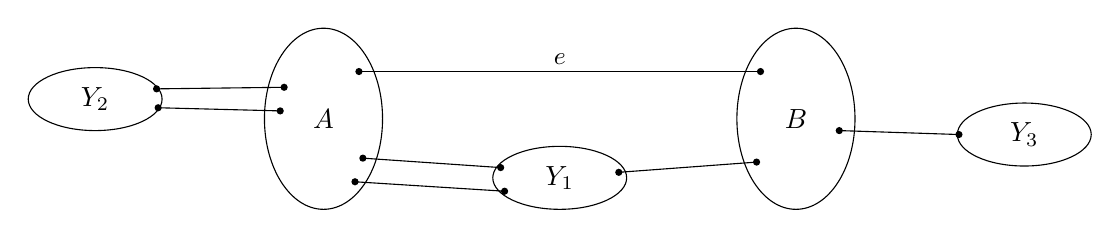
\begin{tikzpicture}
  \draw (0,0) ellipse [x radius=0.75, y radius=1.15];
  \draw (6,0) ellipse [x radius=0.75, y radius=1.15];
  \draw (3,-0.75) ellipse [x radius=0.85, y radius=0.4];
  \draw (-2.9,0.25) ellipse [x radius=0.85, y radius=0.4];
  \draw (8.9,-0.2) ellipse [x radius=0.85, y radius=0.4];
  \node at (0,0) {$A$};
  \node at (6,0) {$B$};
  \node at (3,-0.75) {$Y_1$};
  \node at (-2.9,0.25) {$Y_2$};
  \node at (8.9,-0.2) {$Y_3$};
  \draw (0.45,0.6) -- node[above=-1pt] {\small$e$} (5.55,0.6);
  \draw (0.5,-0.5) -- (2.25,-0.62);
  \draw (0.4,-0.8) -- (2.3,-0.92);
  \draw (5.5,-0.55) -- (3.75,-0.68);
  \draw (-0.5,0.4) -- (-2.12,0.38);
  \draw (-0.55,0.1) -- (-2.1,0.14);
  \draw (6.55,-0.15) -- (8.07,-0.2);
  \foreach \p in {(0.45,0.6),(5.55,0.6),(0.5,-0.5),(2.25,-0.62),(0.4,-0.8),(2.3,-0.92),(5.5,-0.55),
                  (3.75,-0.68),(-0.5,0.4),(-2.12,0.38),(-0.55,0.1),(-2.1,0.14),(6.55,-0.15),(8.07,-0.2)}
    \fill \p circle (1.3pt);
\end{tikzpicture}
\caption{Links between two regions $A$ and $B$. The edge $e$ and the component $Y_1$ of
$G-(A\cup B)$ are links. The components $Y_2$ and $Y_3$ are joined to one region only, so they are
not links. Here $\ell(A,B)=2$. In the proof of Lemma~\ref{lem:link} this is the case $a=b=k=1$
and $e(A,B)=1$.}
\label{fig:links}
\end{figure}

\begin{lemma}[Link formula]\label{lem:link}
Let $A$ and $B$ be disjoint regions of a connected graph $G$. Then
$\PP(\cO_A)=2^{\comp(G-A)-|\delta A|}\ge2^{-|\delta A|}$ and
\[
  \PP(\cO_A\cap\cO_B)=2^{\ell(A,B)-1}\,\PP(\cO_A)\,\PP(\cO_B).
\]
Conditionally on $\cO_A$, the set $\xi\cap E(G[A])$ is uniform on $\Z(G[A])$; conditionally on
$\cO_A\cap\cO_B$, the sets $\xi\cap E(G[A])$ and $\xi\cap E(G[B])$ are independent and uniform on
$\Z(G[A])$ and $\Z(G[B])$.
\end{lemma}

\begin{proof}
The even subgraphs that avoid $\delta A$ are the sums of an even subgraph of $G[A]$ and an even
subgraph of $G-A$. So $\PP(\cO_A)=2^{\beta(G[A])+\beta(G-A)-\beta(G)}$, and counting edges and
vertices shows that the exponent is $\comp(G-A)-|\delta A|$. In the same way
\[
  \PP(\cO_A\cap\cO_B)=2^{\beta(G[A])+\beta(G[B])+\beta(G-A-B)-\beta(G)}
     =2^{\comp(G-A-B)+1-|\delta A|-|\delta B|+e(A,B)},
\]
where $e(A,B)$ is the number of edges between $A$ and $B$. Let $a$, $b$ and $k$ be the numbers of
components of $G-A-B$ that are joined to $A$ only, to $B$ only, and to both. Then
$\comp(G-A-B)=a+b+k$, while $\comp(G-A)=a+1$ and $\comp(G-B)=b+1$, and the formula follows since
$\ell(A,B)=k+e(A,B)$. The conditional laws are read off from the two direct sum decompositions.
\end{proof}

So two cut events are independent when there is one link. They are correlated by a factor of
exactly two when there are two links. The correlation is stronger only for pairs with at least
three links, and the next lemma says that such pairs are rare.

\begin{lemma}[Exceptional partners]\label{lem:exc}
Let $A$ be a region of a connected graph $G$, and let $B_1,\dots,B_k$ be pairwise disjoint regions,
disjoint from $A$, with $\ell(A,B_i)\ge3$ for all $i$. Then $k\le|\delta A|$.
\end{lemma}

\begin{proof}
Contract $A$ to a vertex $a$ and each $B_i$ to a vertex $b_i$, and delete the loops that arise.
This changes neither $d=|\delta A|$ nor the numbers $\ell(A,B_i)$, because the sets $B_j$ with
$j\ne i$ are connected and are contracted inside components of $G-(A\cup B_i)$. Let $F$ be a spanning forest of
$G-a$, and for every edge $e=au$ at $a$ attach a new leaf $\tau_e$ to $u$. Call the resulting forest
$F^{+}$ and its $d$ new leaves \emph{terminals}.

Fix $i$. Every link between $a$ and $b_i$ yields a path of $F^{+}$ from $b_i$ to a terminal. For an
edge $e=ab_i$ it is the edge $b_i\tau_e$. For a component $Y$ of $G-\{a,b_i\}$ joined to both, choose
an edge $e=au$ with $u\in Y$ and take the path of $F^{+}$ from $b_i$ to $\tau_e$; after its first
vertex it stays in $Y\cup\{\tau_e\}$. Paths that come from different links therefore start with
different edges at $b_i$, and the union of any two of them is a path between two terminals. Let
$F^{\circ}\subseteq F^{+}$ be the union of all paths between terminals. As $\ell(a,b_i)\ge3$, the
vertex $b_i$ has degree at least $3$ in $F^{\circ}$. All leaves of $F^{\circ}$ are terminals, and a
forest with at most $d$ leaves has at most $d-2$ vertices of degree at least $3$. Hence $k\le d-2$ if $k\ge1$.
\end{proof}

\begin{lemma}[Many small cuts]\label{lem:smallcuts}
Let $A_1,\dots,A_k$ be pairwise disjoint cyclic regions of a connected graph $G$ with
$|\delta A_i|\le d$ for all $i$. Then
\[
  \PP\bigl(\xi\cap E(G[A_i])\text{ is a forest for every }i\bigr)\;\le\;\frac12+\frac{(d+1)\,2^{d-1}}{k}.
\]
\end{lemma}

\begin{proof}
Let $E_i$ be the event that $\cO_{A_i}$ holds and $\xi\cap E(G[A_i])\ne\emptyset$. On $E_i$ the set
$\xi\cap E(G[A_i])$ is a nonempty even subgraph, hence not a forest, so it suffices to bound
$\PP(Z=0)$ for $Z=\sum_i\mathbf{1}_{E_i}$. By Lemma~\ref{lem:link},
$p_i:=\PP(E_i)=\PP(\cO_{A_i})\bigl(1-2^{-\beta(G[A_i])}\bigr)\ge2^{-d-1}$ and
$\PP(E_i\cap E_j)=2^{\ell(A_i,A_j)-1}p_ip_j$ for $i\ne j$. If $\ell(A_i,A_j)\le2$ this is at most
$2p_ip_j$. Otherwise we use $\PP(E_i\cap E_j)\le p_i$; by Lemma~\ref{lem:exc} this happens for at
most $d$ indices $j$, for each $i$. Hence $\EE Z^{2}\le\mu+2\mu^{2}+d\mu$ with
$\mu=\EE Z\ge k\,2^{-d-1}$, and Lemma~\ref{lem:second} gives the claim.
\end{proof}

\subsection{Reduction to a subcubic graph}

\begin{lemma}\label{lem:reduce}
Let $G$ and $W$ be as in Theorem~\ref{thm:forest}, with $m=|E(W)|$ and $c=\comp(W)$. There are a
connected multigraph $\Gamma$ with $\beta(\Gamma)=r$ and all degrees at most $3$, and a set
$P\subseteq V(\Gamma)$, such that
\begin{enumerate}
\item[\textup{(i)}] every vertex outside $P$ has degree $3$, $|P|\le2m$, and $\Gamma[P]$ has at
most $c$ components;
\item[\textup{(ii)}] $p(G,W)\le\PP\bigl(\xi_\Gamma\cap E(\Gamma-P)\text{ is a forest}\bigr)$, where
$\xi_\Gamma$ is uniform on $\Z(\Gamma)$.
\end{enumerate}
In particular $2r-2\le|V(\Gamma)|\le2r+2m$.
\end{lemma}

\begin{proof}
\emph{Splitting.} Replace every vertex $v$ of degree $d\ge4$ by a path $v^{1}v^{2}\cdots v^{d-2}$.
Distribute the $d$ edges at $v$ along this path in some order: two to $v^{1}$, one to each of
$v^{2},\dots,v^{d-3}$, and two to $v^{d-2}$. If $v\in V(W)$, let the edges of $W$ at $v$ come first
in this order, so that they end in an initial segment $v^{1},\dots,v^{i}$ of the path with
$i<\deg_W(v)$. Let $G'$ be the new graph; its degrees are at most $3$. Let $P$ consist of these
initial segments and of the vertices of $W$ that were not split. Then $|P|\le\sum_v\deg_W(v)=2m$,
every edge of $W$ joins two vertices of $P$, and $G'[P]$ has at most $c$ components.

Contracting the new path edges maps $\Z(G')$ bijectively onto $\Z(G)$, so we may take
$\xi_G=\xi_{G'}\cap E(G)$. Every edge of $G'-P$ is a new path edge or an edge of $E(G)\sm E(W)$. If
$\xi_G\sm E(W)$ is a forest, then so is its union with the set of all new path edges, because
contracting these edges, which form a forest, gives back $\xi_G\sm E(W)$. Hence
$p(G,W)\le\PP\bigl(\xi_{G'}\cap E(G'-P)\text{ is a forest}\bigr)$.

\emph{Cleaning.} As long as possible, delete a vertex of degree one outside $P$, or replace a vertex
of degree two outside $P$ and its two edges by a single edge. An even subgraph avoids a pendant edge
and contains both or none of the two edges at a vertex of degree two, so these operations induce
bijections of the cycle spaces. Let $\Gamma$ be the final multigraph. Each edge of $\Gamma-P$ is a
path of $G'$ all of whose vertices lie outside $P$; so if $\xi_\Gamma$ contains a cycle of
$\Gamma-P$, then the corresponding $\xi_{G'}$ contains a cycle of $G'-P$. This proves~(ii).

Edges with both ends in $P$ are never removed, so the vertices of $P$ keep degree at least two, and
the number of components of the graph induced on $P$ does not increase. The vertices outside $P$ now
have degree exactly $3$. Finally $3|V(\Gamma)|-|P|\le2|E(\Gamma)|\le3|V(\Gamma)|$ and
$|E(\Gamma)|=|V(\Gamma)|+r-1$ give the bounds on $|V(\Gamma)|$.
\end{proof}

\subsection{Parameters, and removing the short cycles}

From now on $\Gamma$ and $P$ are as in Lemma~\ref{lem:reduce}, $\xi=\xi_\Gamma$, and $r$ is large.
All $o(\cdot)$ and $O(\cdot)$ refer to $r\to\infty$ and are uniform in $G$ and $W$. Put
\begin{gather*}
  x=\log r,\qquad y=\log x,\qquad z=\log y,\\
  D=\lfloor x/10\rfloor,\qquad L=\lfloor x\sqrt y\rfloor,\qquad
  s=\lfloor(D-1)/2\rfloor,\qquad\varepsilon=20/z .
\end{gather*}
These numbers have the following roles. We delete cycles of length at most $D$, so the graph that
remains has girth greater than $D$. We count cycles of length at most $L$. A non-backtracking walk
of length $s$ in the remaining graph is determined by its two ends. The number $\varepsilon$ is the
error term of the theorem. These letters keep their meaning until the end of the section.

Recall that $|P|\le2\sqrt r$ and $c\le x/100$. Let $\mathcal{F}$ be the event that
$\xi\cap E(\Gamma-P)$ is a forest. We assume that
\begin{equation}\label{eq:assume}
  \PP(\mathcal{F})>\tfrac12+\varepsilon
\end{equation}
and derive a contradiction. By Lemma~\ref{lem:reduce}(ii) this proves Theorem~\ref{thm:forest}.

Let $\mathcal{Q}$ be a maximal family of pairwise disjoint cycles of $\Gamma-P$ of length at most $D$,
loops and pairs of parallel edges included, and let $S$ be the union of their vertex sets. For
$Q\in\mathcal{Q}$ the set $V(Q)$ is a cyclic region of $\Gamma$ with $|\delta V(Q)|\le|Q|\le D$,
because its vertices have degree $3$. On $\mathcal{F}$ the set $\xi\cap E(\Gamma[V(Q)])$ is a forest
for every $Q$, so Lemma~\ref{lem:smallcuts} and~\eqref{eq:assume} give
$|\mathcal{Q}|<(D+1)2^{D-1}/\varepsilon\le\sqrt r$. Hence $|S|\le D\sqrt r$.

Let $J=\Gamma-(P\cup S)$. By the maximality of $\mathcal{Q}$, $J$ is a simple graph of girth greater
than $D$. It has $v=2r+O(\sqrt r\log r)$ vertices, each of degree $3$ in $\Gamma$, so its
\emph{deficit} satisfies
\begin{equation}\label{eq:deficit}
  d_J:=\sum_{u\in V(J)}\bigl(3-\deg_Ju\bigr)\;\le\;3\bigl(|P|+|S|\bigr)=O(\sqrt r\log r).
\end{equation}

\subsection{Cycles of moderate length}

A walk $u_0u_1\cdots u_\ell$ is \emph{non-backtracking} if $u_{i+1}\ne u_{i-1}$ for $0<i<\ell$. Let
$N_\ell(u,w)$ be the number of non-backtracking walks of length $\ell$ from $u$ to $w$ in $J$.

\begin{lemma}\label{lem:walks}
If $\ell>s$, then $N_\ell(u,w)\le3\cdot2^{\ell-s-1}$ for all $u,w$. Consequently, for every vertex
$u$ of $J$, the cycles $C$ of $J$ through $u$ with $|C|\le L$ satisfy $\sum_C2^{-|C|}\le L\,2^{-s}$.
\end{lemma}

\begin{proof}
There are at most $3\cdot2^{\ell-s-1}$ ways to choose the first $\ell-s$ steps. The last $s$ steps
form a non-backtracking walk of length $s$ between two given vertices. Such a walk is a path,
because $s$ is less than the girth, and there is at most one such path, because two of them would
give a cycle of length at most $2s<D$. For the second statement, a cycle of length $\ell$ through $u$
can be traversed from $u$ in two directions, so there are at most $\half N_\ell(u,u)$ of them, and
$\ell>D>s$.
\end{proof}

Let $B$ be the non-backtracking matrix of $J$. Its rows and columns are indexed by the directed
edges $(i\to j)$ of $J$, two for each edge. The entry in row $(i\to j)$ and column $(j'\to k)$ is
$1$ if $j'=j$ and $k\ne i$, and it is $0$ otherwise.

\begin{lemma}\label{lem:spectrum}
For every even $\ell\ge2$,
\[
  \tr B^{\ell}\;\ge\;\bigl(2-d_J/v\bigr)^{\ell}-3v\,2^{\ell/2}.
\]
\end{lemma}

\begin{proof}
Let $A$ be the adjacency matrix of $J$ and $\Delta$ the diagonal matrix of its degrees, and put
$M(\lambda)=\lambda^{2}I-\lambda A+\Delta-I$.

(1) \emph{If $M(\lambda)g=0$ for a real $\lambda>1$ and a vector $g\ne0$, then $\lambda$ is an
eigenvalue of $B$.} A direct computation shows that $f(i\to j)=\lambda g(j)-g(i)$ satisfies
$Bf=\lambda f$; and $f=0$ would give $g(i)=\lambda g(j)=\lambda^{2}g(i)$ along every edge, hence
$g=0$ (at an isolated vertex, $M(\lambda)g=0$ already says $(\lambda^{2}-1)g=0$).

(2) \emph{If $Bf=\lambda f$ with $f\ne0$ and $\lambda^{2}\ne1$, then $M(\lambda)g=0$ for
$g(j)=\sum_{k\sim j}f(j\to k)$, and $g\ne0$.} The eigenvalue equation at $(i\to j)$ and at
$(j\to i)$ reads $\lambda f(i\to j)=g(j)-f(j\to i)$ and $\lambda f(j\to i)=g(i)-f(i\to j)$.
Eliminating $f(j\to i)$ gives $(\lambda^{2}-1)f(i\to j)=\lambda g(j)-g(i)$. This shows that
$g\ne0$. Summing it over the neighbours $j$ of $i$ gives $M(\lambda)g=0$.

(3) \emph{$B$ has a real eigenvalue $\lambda_1\ge2-d_J/v$.} The matrix
$M(2)=2(\Delta-A)+(3I-\Delta)$ is positive semidefinite, while
$\mathbf{1}^{\!\top}M(\lambda)\mathbf{1}=(\lambda-1)(v\lambda-2v+d_J)$ vanishes at
$\lambda^{*}=2-d_J/v>1$. The smallest eigenvalue of the symmetric matrix $M(\lambda)$ is continuous
in $\lambda$, at most $0$ at $\lambda^{*}$ and at least $0$ at $2$. So $M(\lambda_1)$ is singular for
some $\lambda_1\in[\lambda^{*},2]$, and (1) applies.

(4) \emph{Every non-real eigenvalue $\lambda$ of $B$ satisfies $|\lambda|\le\sqrt2$.} With $g$ as
in~(2), $g^{*}M(\lambda)g=0$ is a quadratic equation $a\lambda^{2}-b\lambda+c'=0$ with real
coefficients $a=g^{*}g>0$, $b=g^{*}Ag$ and $c'=g^{*}(\Delta-I)g\le2a$. Its roots are $\lambda$ and
$\bar\lambda$, so $|\lambda|^{2}=c'/a\le2$.

Now $\tr B^{\ell}$ is the sum of the $\ell$th powers of the $2|E(J)|\le3v$ eigenvalues of $B$. For
even $\ell$ the real eigenvalues contribute nonnegative terms, one of which is at least
$(2-d_J/v)^{\ell}$, and the non-real ones contribute at least $-3v\,2^{\ell/2}$ in total.
\end{proof}

Facts (2) and (4) are part of the Ihara--Bass theory~\cite{Bass,KS}. The test vector $\mathbf{1}$
in~(3) is from~\cite{KNT}. It makes the argument work without any assumption of regularity or
expansion.

\begin{lemma}[Cycle weight]\label{lem:weight}
Let $\mathcal{C}$ be the set of cycles of $J$ of length at most $L$. Their total weight satisfies
\[
  \mu:=\sum_{C\in\mathcal{C}}2^{-|C|}\;\ge\;\bigl(\tfrac18-o(1)\bigr)\ln y .
\]
\end{lemma}

\begin{proof}
$\tr B^{\ell}$ is the number of closed walks $u_0u_1\cdots u_\ell=u_0$ in $J$ with
$u_{i+1}\ne u_{i-1}$ for all $i$ modulo $\ell$. A cycle of length $\ell$ gives $2\ell$ of them; let
$n_\ell$ be the number of the others. Then
\[
  T:=\sum_{\ell\le L}\frac{\tr B^{\ell}}{2\ell\,2^{\ell}}=\mu+\sum_{\ell\le L}\frac{n_\ell}{2\ell\,2^{\ell}} .
\]
Consider a walk counted by $n_\ell$, and let $j$ be the least index with
$u_j\in\{u_0,\dots,u_{j-1}\}$, say $u_j=u_i$. Then $j<\ell$, the walk $C=u_iu_{i+1}\cdots u_j$ is a
cycle, of length $q$ say, and $u_ju_{j+1}\cdots u_\ell u_1\cdots u_i$ is a non-backtracking closed
walk of length $\ell-q>0$ from $u_i$ to itself. It contains a cycle, so $\ell-q>D>s$. The original
walk is determined by $C$, by the vertex $u_i$ and a direction on $C$ ($2q$ choices), by the
complementary walk (at most $3\cdot2^{\ell-q-s-1}$ choices, by Lemma~\ref{lem:walks}), and by the
position of $u_0$ on the latter (at most $\ell$ choices). Hence
\[
  \sum_{\ell\le L}\frac{n_\ell}{2\ell\,2^{\ell}}
  \;\le\;\sum_{\ell\le L}\ \sum_{C\in\mathcal{C}}\tfrac32\,|C|\,2^{-|C|-s}
  \;\le\;\tfrac32\,L^{2}\,2^{-s}\,\mu=o(\mu),
\]
because $2^{-s}\le8\,r^{-1/20}$ and $L^{2}\le x^{2}y$.

On the other hand, for even $\ell$ with $6x\le\ell\le L$, Lemma~\ref{lem:spectrum}
and~\eqref{eq:deficit} give
\[
  2^{-\ell}\tr B^{\ell}\;\ge\;\Bigl(1-\frac{d_J}{2v}\Bigr)^{\ell}-3v\,2^{-\ell/2}
  \;\ge\;1-\frac{L\,d_J}{2v}-3v\,r^{-3}=1-o(1).
\]
All terms of $T$ are nonnegative, so $T\ge(1-o(1))\sum1/(2\ell)$ over the even $\ell$ in $[6x,L]$,
and this sum is $(\frac14-o(1))\ln(L/6x)=(\frac18-o(1))\ln y$. Therefore
$\mu=(1-o(1))T\ge(\frac18-o(1))\ln y$.
\end{proof}

\subsection{The second moment}

For $C\in\mathcal{C}$ let $I_C$ be the event that $C$ is a component of $\xi$. As the vertices of
$C$ have degree $3$ in $\Gamma$, this is the event $E(C)\subseteq\xi$. It is also the event that
$\cO_{V(C)}$ holds and $\xi\cap E(\Gamma[V(C)])=E(C)$. Put
\[
  a_C=2^{-|C|},\qquad p_C=\PP(I_C),\qquad X_C=\frac{a_C}{p_C}\,\mathbf{1}_{I_C},\qquad
  Z=\sum_{C\in\mathcal{C}}X_C .
\]
The factor $a_C/p_C$ fixes the mean of $X_C$ at the combinatorial weight $a_C$, whatever the
probability $p_C$ is. We have no upper bound for $p_C$, and with this normalisation we need none.
The event $I_C$ is given by
$|C|$ linear conditions on $\xi\in\Z(\Gamma)$, which are satisfied by $\xi=C$. So $p_C\ge a_C$.
Hence $0\le X_C\le1$, and $\EE Z=\mu$ with $\mu$ as in Lemma~\ref{lem:weight}. On $\mathcal{F}$
no cycle of $J\subseteq\Gamma-P$ is contained in $\xi$, so $Z=0$, and by~\eqref{eq:assume}
\begin{equation}\label{eq:Zzero}
  \PP(Z=0)>\tfrac12+\varepsilon .
\end{equation}

Let $C\ne C'$ be in $\mathcal{C}$. If they share a vertex, then $I_C\cap I_{C'}=\emptyset$. If they
are disjoint, Lemma~\ref{lem:link}, applied to the regions $V(C)$ and $V(C')$ of $\Gamma$, gives
$\PP(I_C\cap I_{C'})=2^{\ell(C,C')-1}p_Cp_{C'}$ and therefore
\begin{equation}\label{eq:pair}
  \EE(X_CX_{C'})=a_Ca_{C'}\,2^{\ell(C,C')-1},
\end{equation}
where $\ell(C,C')$ is the number of links between $V(C)$ and $V(C')$ in $\Gamma$.

\begin{lemma}[Few links]\label{lem:links}
$\ell(C,C')\le c+o(x)$ for all disjoint $C,C'\in\mathcal{C}$.
\end{lemma}

\begin{proof}
Let $U=V(C)\cup V(C')$. Every vertex of $U$ lies on exactly one edge outside its own cycle, so at
most $2L$ edges leave $U$. At most $c$ components of $\Gamma-U$ meet $P$, because $P\cap U=\emptyset$
and so each component of $\Gamma[P]$ lies in one of them. Let $Y$ run over the other components and
let $d_Y$ be the number of edges between $Y$ and $U$; then $\sum_Yd_Y\le2L$. Put
$t_0=\lfloor y/2\rfloor$.

\emph{Large cuts.} At most $2L/t_0$ components have $d_Y>t_0$.

\emph{Small cuts, cyclic.} The components $Y$ with $d_Y\le t_0$ that are cyclic are pairwise
disjoint cyclic regions inside $\Gamma-P$ with $|\delta Y|\le t_0$. On $\mathcal{F}$ each
$\xi\cap E(\Gamma[Y])$ is a forest, so by Lemma~\ref{lem:smallcuts} and~\eqref{eq:assume} there are
fewer than $(t_0+1)2^{t_0-1}/\varepsilon$ of them.

\emph{Small cuts, trees.} Let $Y$ induce a tree, with $d_Y\le t_0$. No $Q\in\mathcal{Q}$ meets $Y$,
since $Q$ is a connected subgraph of $\Gamma-U$ and would lie in $Y$. Hence $Y\subseteq V(J)$. As
all degrees are $3$, we have $3|Y|=2(|Y|-1)+d_Y$, that is, $|Y|=d_Y-2$. So if $Y$ is joined to both
cycles, there is a path $R$ from $C$ to $C'$ through $Y$ with at most $t_0$ edges. For a link that
is an edge, let $R$ be that edge. The paths $R$ obtained in this way lie in $J$ and are pairwise
disjoint. Divide each of $C$ and $C'$ into at most $8L/D$ blocks of at most $D/4$ consecutive
vertices. If two of the paths had their ends in the same block of $C$ and in the same block of $C'$,
they would form, together with two arcs inside these blocks, a cycle of $J$ of length less than
$2t_0+D/2\le D$. So there are at most $(8L/D)^{2}$ such paths.

Altogether
\[
  \ell(C,C')\;\le\;c+\frac{2L}{t_0}+\frac{(t_0+1)2^{t_0-1}}{\varepsilon}+\Bigl(\frac{8L}{D}\Bigr)^{2}
  =c+O\Bigl(\frac{x}{\sqrt y}\Bigr)+O\bigl(yz\sqrt x\bigr)+O(y)=c+o(x).\qedhere
\]
\end{proof}

\begin{proof}[Proof of Theorem~\ref{thm:forest}]
Call a disjoint pair $C,C'\in\mathcal{C}$ \emph{exceptional} if $\ell(C,C')\ge3$. Fix $C$, and let
$\mathcal{E}$ be a maximal family of pairwise disjoint exceptional partners of $C$. By
Lemma~\ref{lem:exc}, $|\mathcal{E}|\le|\delta V(C)|\le L$, so the union $U_C$ of their vertex sets
has at most $L^{2}$ vertices, and every exceptional partner of $C$ meets $U_C$. By
Lemma~\ref{lem:walks}, the sum of $a_{C'}$ over all $C'\in\mathcal{C}$ that meet $U_C$ is at most
$L^{3}2^{-s}$. With~\eqref{eq:pair} and Lemma~\ref{lem:links},
\[
  \sum_{C'\ \mathrm{exceptional}}\EE(X_CX_{C'})\;\le\;a_C\,2^{c+o(x)}L^{3}\,2^{-s}
  =a_C\,2^{\,c-x/20+o(x)}=o(a_C),
\]
because $c\le x/100$.

For the other disjoint pairs $\EE(X_CX_{C'})\le2a_Ca_{C'}$. Intersecting pairs contribute nothing,
and $\EE X_C^{2}\le\EE X_C=a_C$. Summing over $C$ we get
$\EE Z^{2}\le2\mu^{2}+(1+o(1))\mu$. By Lemmas~\ref{lem:second} and~\ref{lem:weight},
\[
  \PP(Z=0)\;\le\;\frac12+\frac{1+o(1)}{4\mu}\;\le\;\frac12+\frac{2+o(1)}{\ln y}\;<\;\frac12+\frac{20}{z}
\]
for large $r$, since $\ln y=z\ln2$. This contradicts~\eqref{eq:Zzero}.
\end{proof}

\begin{remark}\label{rem:range}
The assumption $|E(W)|\le\sqrt r$ entered only through $|P|\le2\sqrt r$ in~\eqref{eq:deficit}, where
all that is needed is $L\,d_J=o(v)$; the proof therefore works unchanged for
$|E(W)|\le r/\log^{2}r$. Similarly the constant $20$ can be replaced by any constant larger than
$2/\ln2$. We have kept the statement of~\cite{KNT}, which is the one that has been formalised.
\end{remark}
\section{Two elementary theorems}\label{sec:exact}

This section proves Theorem~\ref{thm:exact}. Part~(a) is Proposition~\ref{prop:terminal}, and
part~(b) is Proposition~\ref{prop:nowaste}. Both are formalised (Table~\ref{tab:status}).

Three conditions on a subgraph $W$ of $G$ are easily confused, so we separate them first. Let $W$
have $m\ge1$ edges.
\begin{enumerate}
\item[\textup{(i)}] \emph{Every outside part is a forest.} This means $p(G,W)=1$. It holds if and
only if $G-E(W)$ is a forest: a subset of a forest is a forest, and a cycle of $G-E(W)$ is its own
outside part.
\item[\textup{(ii)}] \emph{No outside part is wasted.} This means that every outside part is the
outside part of some cycle. It is the hypothesis of Proposition~\ref{prop:nowaste}, and it does not
imply~(i). Let $G$ be $K_5$ minus an edge, and let $W$ be the triangle on its three vertices of
degree four. Then $G-E(W)$ is $K_{2,3}$. The sixteen outside parts are the empty set, twelve paths
and three four-cycles. Each of them is the outside part of a cycle, but only thirteen are forests.
So no outside part is wasted, and $p(G,W)=13/16$.
\item[\textup{(iii)}] \emph{Equality in~\eqref{eq:trivial}.} This never holds. The cycles with
empty outside part lie in $W$, so they have fewer than $m$ different lengths. Every other outside
part accounts for at most $m$ lengths. So the cycles of $G$ have fewer than $m\,2^{r-t}$ lengths.
\end{enumerate}
Proposition~\ref{prop:terminal} is about a fourth condition: a graph has the largest possible
number of paths between two vertices.

\subsection{Two terminals}

\begin{proposition}\label{prop:terminal}
Let $N$ be a connected graph and let $u\ne v$ be two of its vertices. Then $N$ has at most
$2^{\beta(N)}$ paths from $u$ to $v$. If it has exactly $2^{\beta(N)}$, then $N-E(A)$ is a forest
for every path $A$ from $u$ to $v$, and every such path has at least $\beta(N)$ edges.
\end{proposition}

\begin{proof}
A path from $u$ to $v$ is a $\{u,v\}$-join in the sense of Example~\ref{rem:twoports}: exactly $u$
and $v$ have odd degree in it. The joins form a coset of $\Z(N)$, so there are $2^{\beta(N)}$ of
them. This proves the first statement. Now suppose that all joins are paths, and let $A$ be one of
them. If $N-E(A)$ contained a cycle $C$, then $A\cup C=A+C$ would be a join that is not a path. So
$N-E(A)$ is a forest. Deleting an edge lowers the rank by at most one, so $\beta(N)\le|A|$.
\end{proof}

Equivalently, an edge $f$ of a graph $G$ lies on at most $2^{\beta(G)-1}$ cycles, and if it lies on
that many, then each of them has at least $\beta(G)$ edges. Equality in
Proposition~\ref{prop:terminal} holds for the necklace $N_j$ of Section~\ref{sec:upper} between
$v_0$ and $v_j$. It also holds for $K_4$ minus an edge and for $K_{3,3}$ minus an edge, in each case
between the ends of the deleted edge.

This explains the shape of the construction. The necklace $N_k$ turns $k$ units of rank into
$2^{k}$ path lengths, the most that $k$ units can give. By Proposition~\ref{prop:terminal}, no
gadget that does this has a path with fewer than $k$ edges between its terminals. So the cycles
through $N_k$ have length greater than $k$, and the lengths $3,\dots,k$ must be produced elsewhere.
The construction uses a necklace with about $\log k$ beads for them. Its own short lengths require
a third necklace, and so on.

Each of these necklaces costs a factor of two. Consider a necklace $N_j$ that is closed by a chord
$f_j$, together with $f_j$ and the chords of the smaller necklaces. Call this part $W$. The rest of
the graph is attached to $W$ at the two vertices $v_0$ and $v_j$ only. By
Example~\ref{rem:twoports}, half of the outside parts are even subgraphs of the rest. A cycle that
uses an edge of $W$ cannot have a nonempty even subgraph as its outside part. So nearly half of the
outside parts are of no use to the cycles through $W$. These $\lgs k$ halvings are the term
$\lgs n$ of Theorem~\ref{thm:main}.

\paragraph{Formal counterpart.}
Proposition~\ref{prop:terminal} is the theorem \lean{twoTerminalTheorem}. The formal statement also
covers the case $u=v$. The formal proof gets the bound $\beta(N)\le|A|$ from a count: an even
subgraph of $N$ is determined by its edges on the path $A$.

\subsection{No waste}

Lemma~\ref{lem:count} counts the cycles of $G$ by their outside parts. Recall that an outside
part is \emph{wasted} if it is not the outside part of any cycle. A graph cannot avoid all waste
for long.

\begin{proposition}\label{prop:nowaste}
Let $G$ be a connected graph and let $W\subseteq G$ be a subgraph that contains a cycle. Suppose
that no outside part is wasted. Then every nonempty even subgraph of $G-E(W)$ is a cycle, and
\[
  \beta(G)-\beta(W)\;\le\;|V(W)|+3 .
\]
\end{proposition}

\begin{proof}
Let $z$ be a nonempty even subgraph of $G-E(W)$. Then $z$ is its own outside part. By assumption
some cycle $C$ has outside part $z$, so $z\subseteq C$. A cycle that contains a nonempty even
subgraph is equal to it. So $z$ is a cycle.

In particular, two edge-disjoint cycles of $G-E(W)$ would have a union that is an even subgraph but
not a cycle. So the graph $G'=G-E(W)$, on the vertex set $V(G)$, has no two edge-disjoint cycles.
By Lemma~\ref{lem:EP} below, $|E(G')|\le|V(G)|+3$. Now $\beta(G)=|E(G)|-|V(G)|+1$ and
$\beta(W)\ge|E(W)|-|V(W)|+1$. Hence
$\beta(G)-\beta(W)\le|E(G')|-|V(G)|+|V(W)|\le|V(W)|+3$.
\end{proof}

\begin{lemma}[Erd\H{o}s and P\'osa~\cite{EP}]\label{lem:EP}
A multigraph with $n$ vertices and at least $n+4$ edges contains two edge-disjoint cycles.
\end{lemma}

\begin{proof}
We include the short proof. Let $H$ be a counterexample with $|V(H)|+|E(H)|$ minimal, and let $n$
be its number of vertices. Then $H$ has exactly $n+4$ edges and no vertex of degree at most one. It
has no vertex of degree two either. If such a vertex carries a loop, then the rest of $H$ contains a
second cycle. Otherwise the vertex and its two edges can be replaced by a single edge, which gives a
smaller counterexample. So
$2(n+4)\ge3n$, that is, $n\le8$. Let $C$ be a shortest cycle of $H$. Since $H-E(C)$ is a forest,
$n+4-|C|\le n-1$, so $|C|\ge5$. Thus $H$ is a simple graph of minimum degree at least $3$ and girth
at least $5$, and such a graph has at least $1+3+6=10$ vertices, a contradiction.
\end{proof}

A graph in which every nonempty even subgraph is a cycle has $2^{\beta}-1$ cycles, the largest
possible number. Such graphs are known. Entringer and Slater~\cite[Theorem~1]{ES} quote a theorem of
Maurer, and of Mateti and Deo: a connected graph has this property if and only if it reduces to
$K_1$, $K_3$, $K_4$ minus an edge, $K_4$ or $K_{3,3}$. A reduction deletes a vertex of degree one,
or suppresses a vertex of degree two whose two neighbours are not adjacent. So the first conclusion of Proposition~\ref{prop:nowaste}
puts $G-E(W)$ into a known class. In the language of codes, a binary code in which every nonzero
word is minimal is intersecting~\cite[\S2]{AACST}.

The second conclusion is sharp up to the additive constant. If $W$ is a cycle $w_1\cdots w_m$ and
$G$ consists of $W$ and a path of length two from $w_i$ to $w_{i+1}$ for every $i$ modulo $m$, then
no outside part is wasted and $\beta(G)-\beta(W)=|V(W)|$. In the example of~(ii) above,
$\beta(G)-\beta(W)=|V(W)|+1$. An exhaustive search found nothing better for a triangle $W$ in
graphs with at most eight vertices.

\paragraph{Formal counterpart.}
Proposition~\ref{prop:nowaste} is the theorem \lean{noWasteTheorem}. There $W$ is given by its edge
set $S$, and $\beta(W)$ is defined through the graph on all vertices of $G$ with edge set $S$.
Lemma~\ref{lem:EP} is the theorem \lean{ExactCounting.Multi.card_le_of_intersecting}. It is stated
for multigraphs in the language of even edge sets: if any two nonempty even edge sets share an
edge, then there are at most $n+3$ edges. The formal proof uses the same reductions as the proof
above. In the last step it finds both even sets by a pigeonhole count.
\section{Problems}\label{sec:problems}

\paragraph{Error terms.}
The error terms in Theorems~\ref{thm:cycles} and~\ref{thm:forest} are of order $1/\lgk3r$. The
truth may be much smaller. By Example~\ref{rem:twoports} the left side of~\eqref{eq:forest} can be
as large as $\half+2^{1-r}$, and Horak and Kim~\cite{HK} proved that
$\psi(r)\ge2^{r-1}+c\,r\,2^{r/2}$. We know no examples with larger error terms.

The weak error term has a definite cause in the proof. The gain $\mu$ comes from cycles with between
$6\log r$ and $\log r\sqrt{\log\log r}$ edges. Each length $\ell$ in this range contributes about
$1/(2\ell)$ to $\mu$. Lemma~\ref{lem:links} dictates the upper end of the range. So the lower bound for $\mu$
that the proof gives is only of order $\lgk3r$.

\begin{problem}
Is the error term in~\eqref{eq:forest} at most $r^{-c}$ for some $c>0$? Is
$\psi(r)\le2^{r-1}+2^{(1-c)r}$?
\end{problem}

\paragraph{Between exactness and the forest estimate.}
Proposition~\ref{prop:nowaste} and Theorem~\ref{thm:forest} both limit how well the cycles of $G$
can use the outside parts, at two different scales. No outside part is wasted for at most
$|V(W)|+3$ ranks beyond $W$. Let $W$ be a union of cycles with at most $(\log r)/100$ components.
Then about half of the outside parts fail to be forests once $r\ge|E(W)|^{2}$, or already once
$r\ge|E(W)|\log^{2}r$ by Remark~\ref{rem:range}. We know no proof of the factor $\half$ that avoids the second moment
computation of Section~\ref{sec:forest}, except in special cases such as
Example~\ref{rem:twoports}. A stability version of Proposition~\ref{prop:terminal} would be a step
in that direction.

\begin{problem}
Let $\varepsilon>0$. If a connected graph $N$ has at least $(\half+\varepsilon)2^{\beta(N)}$ paths
between two vertices $u$ and $v$, must each of these paths have at least $c(\varepsilon)\beta(N)$
edges?
\end{problem}

\begin{problem}
Can the constant $3$ in Proposition~\ref{prop:nowaste} be replaced by $1$?
\end{problem}

\appendix

\section{The formal statements}\label{app:lean}

The Lean~4 code is in the repository~\cite{Repo}. This paper refers to commit
\texttt{9de7271} on the branch \texttt{feat/cycle-count-bound}. The code uses Lean v4.19.0 and a
pinned revision of Mathlib. It has $264$ modules and $44{,}082$ lines. The nine modules in
\lean{Erdos1016/CycleCount/} have $1{,}554$ lines and contain the proof of
Theorem~\ref{thm:cycles}. The eight modules in \lean{Erdos1016/ExactCounting/} have $1{,}571$
lines and contain the proof of Theorem~\ref{thm:exact}. The rest is the formalisation
from~\cite{KNT}.

\subsection{The statements behind Theorem~\ref{thm:cycles}}

The following text is copied from \lean{Erdos1016/CycleCount/Statement.lean},
\lean{Asymptotic.lean} and \lean{Erdos1016/Main.lean}, without the comments and the proofs.

{\small
\begin{alltt}
def cycleEdgeSets \{V : Type*\} (G : SimpleGraph V) : Set (Set (Sym2 V)) :=
  \{s | \(\exists\) (v : V) (p : G.Walk v v), p.IsCycle \(\land\) s = \{a | a \(\in\) p.edges\}\}

def numCycles \{V : Type*\} (G : SimpleGraph V) : \(\mathbb{N}\) := (cycleEdgeSets G).ncard

def CycleCountStatement : Prop :=
  \(\exists\) r\(\sb{1}\) : \(\mathbb{N}\), \(\forall\) (n : \(\mathbb{N}\)) (G : SimpleGraph (Fin n)) (r : \(\mathbb{N}\)),
    r + n = Nat.card G.edgeSet + Nat.card G.ConnectedComponent \(\to\) r\(\sb{1}\) \(\le\) r \(\to\)
    (numCycles G : \(\mathbb{R}\)) \(\le\)
      (1 / 2 + 21 / Real.logb 2 (Real.logb 2 (Real.logb 2 (r : \(\mathbb{R}\))))) * 2 ^ r

def cycleCounts (r : \(\mathbb{N}\)) : Set \(\mathbb{N}\) :=
  \{c | \(\exists\) (n : \(\mathbb{N}\)) (G : SimpleGraph (Fin n)),
    r + n = Nat.card G.edgeSet + Nat.card G.ConnectedComponent \(\land\) numCycles G = c\}

def maxCycles (r : \(\mathbb{N}\)) : \(\mathbb{N}\) := sSup (cycleCounts r)

def AsymptoticCycleCount : Prop :=
  Tendsto (fun r : \(\mathbb{N}\) => (maxCycles r : \(\mathbb{R}\)) / 2 ^ r) atTop (\(\mathcal{N}\) (1 / 2))

theorem cycleCountTheorem : CycleCount.CycleCountStatement
theorem cycleCountAsymptotic : CycleCount.AsymptoticCycleCount
\end{alltt}}

Four remarks help to compare this with Theorem~\ref{thm:cycles}.
\begin{itemize}
\item \lean{SimpleGraph}, \lean{Walk} and \lean{IsCycle} are Mathlib's. A walk with \lean{IsCycle}
is a closed walk of length at least $3$ that repeats no vertex except its start. The set
\texttt{cycleEdgeSets G} contains the edge set of each such walk once. So \texttt{numCycles G} is the
number of cycles in the sense of this paper, and not the number of closed walks.
\item The hypothesis \texttt{r + n = ...} says that $r=\beta(G)$. It avoids subtraction of natural
numbers.
\item The threshold is existentially quantified, as $r_1$ is in the text. In the proof it is
$\max(r_0,2^{2048})$, where $r_0$ is the threshold of the forest estimate.
\item In Lean, \lean{sSup} of an empty or unbounded set of natural numbers is $0$. This does not
make \lean{maxCycles} degenerate. The code proves that \texttt{cycleCounts r} is bounded by $2^{r}$
(\lean{cycleCounts_bddAbove}) and that its supremum is attained for $r\ge3$ (\lean{maxCycles_mem}).
\end{itemize}
The theorem \lean{cycleCountTheorem_general} states the same bound for simple graphs on every
finite vertex type.

\subsection{The statements behind Theorem~\ref{thm:exact}}

The following text is copied from \lean{Erdos1016/ExactCounting/TwoTerminals.lean},
\lean{NoWaste.lean} and \lean{Erdos1016/Main.lean}, without the comments and the proofs.

{\small
\begin{alltt}
def pathEdgeSets \{V : Type*\} (G : SimpleGraph V) (u v : V) : Set (Set (Sym2 V)) :=
  \{s | \(\exists\) p : G.Walk u v, p.IsPath \(\land\) s = \{a | a \(\in\) p.edges\}\}

def numPaths \{V : Type*\} (G : SimpleGraph V) (u v : V) : \(\mathbb{N}\) := (pathEdgeSets G u v).ncard

def TwoTerminalStatement : Prop :=
  \(\forall\) (n : \(\mathbb{N}\)) (G : SimpleGraph (Fin n)) (r : \(\mathbb{N}\)) (u v : Fin n),
    G.Connected \(\to\) r + n = Nat.card G.edgeSet + 1 \(\to\)
      numPaths G u v \(\le\) 2 ^ r \(\land\)
      (numPaths G u v = 2 ^ r \(\to\)
        \(\forall\) p : G.Walk u v, p.IsPath \(\to\)
          r \(\le\) p.length \(\land\) (G.deleteEdges \{a | a \(\in\) p.edges\}).IsAcyclic)

def IsEvenEdgeSet \{V : Type*\} (s : Set (Sym2 V)) : Prop :=
  \(\forall\) v : V, Even \{e | e \(\in\) s \(\land\) v \(\in\) e\}.ncard

def NoWasteStatement : Prop :=
  \(\forall\) (n : \(\mathbb{N}\)) (G : SimpleGraph (Fin n)) (S : Set (Sym2 (Fin n))) (r t : \(\mathbb{N}\)),
    G.Connected \(\to\) S \(\subseteq\) G.edgeSet \(\to\)
    r + n = Nat.card G.edgeSet + 1 \(\to\)
    t + n = S.ncard + Nat.card (SimpleGraph.fromEdgeSet S).ConnectedComponent \(\to\)
    (\(\forall\) s : Set (Sym2 (Fin n)), s \(\subseteq\) G.edgeSet \(\to\) IsEvenEdgeSet s \(\to\)
      \(\exists\) c \(\in\) CycleCount.cycleEdgeSets G, c \textbackslash{} S = s \textbackslash{} S) \(\to\)
    (\(\forall\) c\(\sb{1}\) \(\in\) CycleCount.cycleEdgeSets (G.deleteEdges S),
      \(\forall\) c\(\sb{2}\) \(\in\) CycleCount.cycleEdgeSets (G.deleteEdges S), \(\lnot\) Disjoint c\(\sb{1}\) c\(\sb{2}\)) \(\land\)
    r \(\le\) t + \{v | \(\exists\) e \(\in\) S, v \(\in\) e\}.ncard + 3

theorem twoTerminalTheorem : ExactCounting.TwoTerminalStatement
theorem noWasteTheorem : ExactCounting.NoWasteStatement
\end{alltt}}

Five remarks help to compare this with Theorem~\ref{thm:exact}.
\begin{itemize}
\item A walk with \lean{IsPath} repeats no vertex. A path is counted once, by its edge set.
\item The graph \texttt{G.deleteEdges s} is $G$ without the edges in \texttt{s}, and
\lean{IsAcyclic} says that it is a forest.
\item The first statement does not assume $u\ne v$.
\item In the second statement \texttt{S} is $E(W)$. The line with \texttt{t} says that $t$ is the
rank of the graph with edge set $S$ on all $n$ vertices. Isolated vertices do not change the rank,
so $t=\beta(W)$. The set in the last line is $V(W)$.
\item Theorem~\ref{thm:exact}(b) assumes that $W$ contains a cycle. The formal statement does not
need this hypothesis: it follows from the main hypothesis for the empty even set.
\end{itemize}

\subsection{The forest estimate}

Theorem~\ref{thm:forest} is the theorem \lean{ShortProof.fewComponentForestEstimate}, which has the
following type.

{\small
\begin{alltt}
def FewComponentForestEstimate : Prop :=
  \(\exists\) rmin : \(\mathbb{N}\), \(\forall\) (G : PhysicalGraph), G.IsConnected \(\to\) rmin \(\le\) G.cycleRank \(\to\)
    \(\forall\) F : Finset G.CycleWord, F.Nonempty \(\to\)
      (witnessSupportEdges G F).card ^ 2 \(\le\) G.cycleRank \(\to\)
      100 * (Nat.card (cycleUnionGraph G F).ConnectedComponent : \(\mathbb{R}\)) \(\le\)
        Real.logb 2 (G.cycleRank : \(\mathbb{R}\)) \(\to\)
      outsideForestProbability G (witnessSupportEdges G F) \(\le\)
        (1 / 2 : \(\mathbb{R}\)) + 20 / tripleLog G.cycleRank
\end{alltt}}

Here \lean{PhysicalGraph} is the project's type of finite simple graphs with numbered vertices and
edges. The family \lean{F} is a nonempty finite set of cycles of \lean{G}, and $W$ is their union.
The set \texttt{witnessSupportEdges G F} is $E(W)$. The graph \texttt{cycleUnionGraph G F} is $W$ on
the vertices that the cycles meet. The number \texttt{outsideForestProbability G E} is the number of
even subgraphs $x$ such that $x\sm E$ is a forest, divided by $2^{\beta(G)}$. Finally
\texttt{tripleLog r} is $\lgk3r$. The statement of Theorem~\ref{thm:main} in Lean is described
in~\cite[\S1.2]{KNT}.

\subsection{Repeating the check}

The repository contains a verifier. It rebuilds every module from source. It compares the types of
the endpoint theorems with statements that are written out a second time in
\lean{audits/TheoremAudit.lean}. It prints the axioms of $65$ declarations, among them all endpoints
in Table~\ref{tab:status}, and it accepts only \lean{propext}, \lean{Classical.choice} and
\lean{Quot.sound}. It rejects proofs that contain \lean{sorry}. The commands are:

{\small
\begin{verbatim}
git clone https://github.com/JWKNT/erdos1016.git && cd erdos1016
git checkout 9de7271abf559dc69c1fd843d043fb504480eac4
elan toolchain install leanprover/lean4:v4.19.0
lake exe cache get
python3 -m unittest discover -s scripts -p 'test_*.py'
python3 scripts/verify.py --fresh --jobs 2
\end{verbatim}}

On 10 November 2026 this check passed for the commit above on a machine of the authors, with a
clean working tree. The repository's continuous integration repeated the check on the same day for
commit \texttt{e45a40b}. That commit differs from \texttt{9de7271} only in the folder
\lean{paper/cycle-count}, so the Lean sources, the audit and the scripts are the same. GitHub
Actions run
\href{https://github.com/JWKNT/erdos1016/actions/runs/42896694067}{42896694067} records the
result.

\subsection{Steps of the proofs}

Table~\ref{tab:steps} names the Lean declaration for each step. Namespaces are omitted, and files
are relative to \lean{Erdos1016/}. The rows for Section~\ref{sec:cycles} match the text closely,
with four differences. The formal proof of Lemma~\ref{lem:indep} uses no spanning tree: it chooses
the edges of $D$ one at a time, and it records only that each of them lies in an even subgraph. The
formal proof uses $r\le\beta(G^{+})\le r+a$ in place of the equality. It states
Lemma~\ref{lem:through} together with the count of the cycles that avoid $D$. It writes $k$ as
$\lfloor\log\lfloor\log r\rfloor\rfloor+1$, which is the same number.

The rows for Section~\ref{sec:exact} match the text, with the differences that are stated at the
end of Sections~\ref{sec:exact}.1 and~\ref{sec:exact}.2.

The rows for Sections~\ref{sec:lower} to~\ref{sec:forest} are taken from~\cite[Appendix~A]{KNT}. We
checked that these declarations exist at the commit above. We did not compare each of them with our
wording. In these parts the formal proof replaces $O$-terms by explicit constants, and intermediate
estimates differ in detail from the text. The statements of Theorems~\ref{thm:forest}
and~\ref{thm:main}, of Proposition~\ref{prop:halving} and of Corollary~\ref{cor:phi} agree with
the Lean statements.

\begin{center}\begin{minipage}{\linewidth}\centering\small
\captionof{table}{Steps of the proofs and the corresponding Lean declarations.}\label{tab:steps}
\smallskip
\renewcommand{\arraystretch}{1.0}
\begin{tabular}{@{}L{3.7cm}L{6.3cm}L{5.6cm}@{}}
\toprule
In this paper & Declaration & File \\
\midrule
Lemma~\ref{lem:indep} & \lean{exists_independent_edges} & \lean{CycleCount/IndependentEdges} \\
Second neighbours & \lean{exists_apex} & \lean{CycleCount/IndependentEdges} \\
Chords and triangles & \lean{addChords}, \lean{cycleRank_addChords_le}, \lean{exists_triangle_family}
  & \lean{CycleCount/ChordExtension}, \lean{CycleCount/TriangleFamily} \\
Lemma~\ref{lem:through} & \lean{card_cycleWord_le} & \lean{CycleCount/ConnectedBound} \\
Theorem~\ref{thm:cycles}, parameters & \lean{witness_parameters},
  \lean{cycleCountBound_of_forestEstimate} & \lean{CycleCount/Bound} \\
Theorem~\ref{thm:cycles}, Mathlib form & \lean{cycleCountStatement_of_bound} &
  \lean{CycleCount/Statement} \\
Lower bound $\psi(r)\ge2^{r-1}$ & \lean{exists_graph_many_cycles} & \lean{CycleCount/LowerBound} \\
$\psi(r)\sim2^{r-1}$ & \lean{asymptoticCycleCount_of_statement} & \lean{CycleCount/Asymptotic} \\
\midrule
Lemma~\ref{lem:witness} & \lean{exists_budgeted_witness} & \lean{Extremal/Witness/CapacityBudget} \\
Proposition~\ref{prop:halving} & \lean{recurrence_of_few_component_forest_estimate} &
  \lean{Extremal/Recurrence/WitnessReduction} \\
Corollary~\ref{cor:phi} & \lean{recurrence_logStar_bound} &
  \lean{Extremal/Recurrence/LinearExponentialDecay} \\
Proposition~\ref{prop:upper} & \lean{upper_bound_integer} & \lean{Extremal/UpperBound} \\
\midrule
Lemma~\ref{lem:link} & \lean{multigraph_zeroCut_pair} &
  \lean{CycleSpace/Graphical/MultigraphCutCorrelation} \\
Lemma~\ref{lem:exc} & \lean{exceptional_partner_card_le} &
  \lean{CycleSpace/Graphical/DisjointRegionCuts} \\
Lemma~\ref{lem:smallcuts} & \lean{smallCut_forest_bound} &
  \lean{Probability/Moments/SmallCutRegionBound} \\
Lemma~\ref{lem:reduce} & \lean{exists_marked_subcubic_reduction} &
  \lean{Graph/Cubicization/MarkedReduction} \\
Lemma~\ref{lem:spectrum} & \lean{normalized_even_trace_lower} &
  \lean{Nonbacktracking/Spectrum/DeficitTrace} \\
Lemma~\ref{lem:weight} & \lean{cycleWordMass_ge_log_ratio} &
  \lean{Cycles/Counting/LowDegreeTraceCycles} \\
Lemma~\ref{lem:links} & \lean{actual_cycle_links_le} & \lean{Cycles/Geometry/ActualCycleLinkBound} \\
Theorem~\ref{thm:forest} & \lean{second_moment_le}, \lean{forest_le_half_add_twenty},
  \lean{fewComponentForestEstimate} & \lean{Probability/Moments/SeedFamilyAvoidance},
  \lean{Probability/Avoidance/FewComponentForest} \\
\midrule
Paths and cycles in Section~\ref{sec:exact} & \lean{par_edges_of_isTrail}, \lean{eq_empty_of_subset_path},
  \lean{eq_edges_of_subset_cycle} & \lean{ExactCounting/EdgeParity} \\
Proposition~\ref{prop:terminal} & \lean{card_even_le_two_pow}, \lean{twoTerminalStatement} &
  \lean{ExactCounting/EvenSets}, \lean{ExactCounting/TwoTerminals} \\
Lemma~\ref{lem:EP} & \lean{exists_even_subset}, \lean{intersecting_suppress},
  \lean{exists_small_dense}, \lean{card_le_of_intersecting} & \lean{ExactCounting/Multigraph},
  \lean{Suppression}, \lean{ShortCycle}, \lean{DisjointCycles} \\
Proposition~\ref{prop:nowaste} & \lean{noWasteStatement} & \lean{ExactCounting/NoWaste} \\
\bottomrule
\end{tabular}
\end{minipage}\end{center}

\section{Tests on small graphs}\label{app:checks}

We tested the examples of this paper, and our wording of the proofs, on small graphs. The scripts
are in the folder \lean{paper/cycle-count/paper-checks} of the repository~\cite{Repo}, at commit
\texttt{e45a40b}. They use
exact arithmetic, except for the two scripts on the non-backtracking matrix, which compute
eigenvalues in floating point. All tests passed. A passed test is evidence, not a proof.

\begin{itemize}
\item \emph{The examples} (\lean{check_examples.py}). The numbers in Example~\ref{rem:twoports},
the ring of four-cycles in Section~\ref{sec:cycles} for $2\le j\le7$, the example in~(ii) of
Section~\ref{sec:exact}, and the cycle with ears in Section~\ref{sec:exact} for $3\le m\le6$.
\item \emph{Section~\ref{sec:cycles}} (\lean{check_chords.py}). $300$ random connected graphs with
$4$ to $8$ vertices and every admissible $k$, which gives $857$ cases. The script takes $D$ outside a
random spanning tree and builds the chords, $G^{+}$ and $W$. It checks Lemmas~\ref{lem:indep}
and~\ref{lem:through}, the existence of the second neighbours, and the stated properties of
$G^{+}$ and $W$.
\item \emph{Lemma~\ref{lem:count} and Proposition~\ref{prop:nowaste}}
(\lean{check_counting.py}). $4000$ random connected graphs with $4$ to $8$ vertices, each with a
random subgraph $W$. The script checks the number of outside parts, the bound of
Lemma~\ref{lem:count}(b), and the bound $2^{r}p+2^{r-t}(1-p)$ on the number of all cycles, which follows from the proof of
that lemma. In the
$2027$ cases without a wasted outside part it checks both conclusions of
Proposition~\ref{prop:nowaste}.
\item \emph{Proposition~\ref{prop:nowaste}, exhaustively} (\lean{nowaste_exh.py},
\lean{nowaste_exh2.py}). For connected $W$ we have
$\beta(G)-\beta(W)-|V(W)|=|E(G)\sm E(W)|-|V(G)|$. The scripts enumerate connected graphs $G$
that contain a fixed triangle $W$. They cover all such graphs with $5$ or $6$ vertices. For $7$
vertices they cover the graphs with at least $8$ edges outside $W$, and for $8$ vertices those with
at least $10$. For a fixed four-cycle $W$ they cover all graphs with $6$ vertices, and the graphs
with $7$ vertices and at least $8$ edges outside $W$. Graphs with more than $|V(G)|+3$ edges outside $W$ are skipped, because
Lemma~\ref{lem:EP} excludes them. Without a wasted outside part, the largest value of
$\beta(G)-\beta(W)-|V(W)|$ was $1$ for the triangle and $0$ for the four-cycle.
\item \emph{Proposition~\ref{prop:upper}} (\lean{check_construction.py}). The graph of
Section~\ref{sec:upper} for all $n\le139$ and for $n\in\{263,264,265,300,500,520,521,522\}$. Each
graph is pancyclic, and the number of chords never exceeds $\lfloor\log n\rfloor+\lgs n+1$.
\item \emph{Lemmas~\ref{lem:link} and~\ref{lem:exc}} (\lean{check_links.py}). $400$ random connected
multigraphs with $5$ to $9$ vertices and $5221$ pairs of disjoint regions with at most three
vertices each. The script checks the link formula and the bound on exceptional partners.
\item \emph{Lemmas~\ref{lem:walks} and~\ref{lem:spectrum}} (\lean{check_nb.py},
\lean{check_nb2.py}). $292$ random graphs of maximum degree $3$ with $10$ to $40$ vertices, and the
Petersen, Heawood and Tutte--Coxeter graphs. The scripts check the walk bound, the two statements
on eigenvalues, and the trace inequality for even $\ell\le24$.
\end{itemize}

\section{Sources}\label{app:sources}

We compared the bibliographic data of every reference with the publisher's record, with Crossref
or with arXiv. For~\cite{ES} we used the scan that is linked from the OEIS. We
read~\cite{AACST}, \cite{ES}, \cite{Griffin}, \cite{KNT}, and the parts of~\cite{HK} that concern
cycles. Of~\cite{AT} we read the abstract. We have not seen~\cite{Bass}, \cite{Bondy},
\cite{EP} or~\cite{KS}. What we say about~\cite{Bondy} is taken from~\cite{Bloom}
and~\cite{KNT}. No proof in this paper depends on a source that we have not seen. The lemma
from~\cite{EP} is proved in Section~\ref{sec:exact}, and the facts related to~\cite{Bass,KS} are
proved in Section~\ref{sec:forest}.

We looked for an earlier proof of $\psi(r)\sim2^{r-1}$, and for any bound below
$\frac{15}{16}2^{r}$ for cubic graphs. We used web searches and the literature discussed
in~\cite{AACST} and~\cite{HK}, and we found neither. A search of this kind can miss things.

The two theorems of Section~\ref{sec:exact} are elementary, and they are close to known results.
Lemma~\ref{lem:EP} is due to Erd\H{o}s and P\'osa. The graphs in which every nonempty even subgraph
is a cycle were characterised by Maurer and by Mateti and Deo; we know this
from~\cite[Theorem~1]{ES} and have not seen the original papers. We do not know whether
Proposition~\ref{prop:terminal} or the bound in Proposition~\ref{prop:nowaste} has been stated
before.

The repository keeps three earlier drafts of this paper and the notes of the search for a simpler
proof, next to the manuscript in the folder \lean{paper/cycle-count}.

\begin{thebibliography}{99}\small

\bibitem{AACST} A.~Alahmadi, R.~E.~L.~Aldred, R.~dela~Cruz, P.~Sol\'e and C.~Thomassen, The maximum
number of minimal codewords in long codes, \emph{Discrete Appl.\ Math.}\ \textbf{161} (2013),
424--429. arXiv:1201.6043.

\bibitem{AT} R.~E.~L.~Aldred and C.~Thomassen, On the maximum number of cycles in a planar graph,
\emph{J.~Graph Theory} \textbf{57} (2008), 255--264.

\bibitem{Bass} H.~Bass, The Ihara--Selberg zeta function of a tree lattice, \emph{Internat.\
J.~Math.}\ \textbf{3} (1992), 717--797.

\bibitem{Bloom} T.~F.~Bloom, Erd\H{o}s Problem \#1016, \url{https://www.erdosproblems.com/1016},
accessed November 2026.

\bibitem{Bondy} J.~A.~Bondy, Pancyclic graphs~I, \emph{J.~Combin.\ Theory Ser.~B} \textbf{11}
(1971), 80--84.

\bibitem{ES} R.~C.~Entringer and P.~J.~Slater, On the maximum number of cycles in a graph,
\emph{Ars Combin.}\ \textbf{11} (1981), 289--294. A scan is linked from the entry A006188 of the
OEIS, \url{https://oeis.org/A006188}.

\bibitem{EP} P.~Erd\H{o}s and L.~P\'osa, On the maximal number of disjoint circuits of a graph,
\emph{Publ.\ Math.\ Debrecen} \textbf{9} (1962), 3--12.

\bibitem{Griffin} S.~Griffin, Minimal pancyclicity, arXiv:1312.0274 (2013).

\bibitem{HK} P.~Horak and D.~Kim, Connected cubic graphs with the maximum number of perfect
matchings, \emph{J.~Graph Theory} \textbf{99} (2022), 671--690. arXiv:2006.13459.

\bibitem{KNT} KNT, The minimum number of edges in a pancyclic graph, manuscript, September 2026,
\url{https://jehlp.net/erdos1016/}.

\bibitem{Claim} KNT, Proof claim for Problem \#1016, Erd\H{o}s Problems forum, 24 September 2026,
\url{https://www.erdosproblems.com/forum/thread/1016/proof-claims}, accessed November 2026.

\bibitem{Repo} KNT, Astra and Fable~5.2, Lean~4 formalisation of the results of~\cite{KNT} and of
this paper, \url{https://github.com/JWKNT/erdos1016}.

\bibitem{KS} M.~Kotani and T.~Sunada, Zeta functions of finite graphs, \emph{J.~Math.\ Sci.\ Univ.\
Tokyo} \textbf{7} (2000), 7--25.

\bibitem{Lean4} L.~de~Moura and S.~Ullrich, The Lean~4 theorem prover and programming language,
in: \emph{CADE~28}, Lecture Notes in Comput.\ Sci.\ \textbf{12699}, Springer, 2021, 625--635.

\bibitem{Mathlib} The mathlib Community, The Lean mathematical library, in: \emph{CPP~2020}, ACM,
2020, 367--381.

\end{thebibliography}

\end{document}
